\begin{singlespacing}
\chapter{A search for new phenomena}
\label{chapter:2ljets}
%
\begin{epigraphs}
\qitem{%
An experiment is never a failure solely because it fails to
achieve predicted results. An experiment is a failure only when it also
fails adequately to test the hypothesis in question, when the data it
produces don’t prove anything one way or another.%
}%
{Robert~M.~Pirsig,
\textit{Zen and the Art of Motorcycle Maintenance},
1974~\cite{pirsig1999zen}}
\qitem{%
But there is one feature I notice that is generally missing in cargo cult
science. \ldots\
% That is the idea that we all hope you have learned in studying science in
% school--we never say explicitly what this is, but just hope that you catch
% on by all the examples of scientific investigation. It is interesting,
% therefore, to bring it out now and speak of it explicitly.
It's a kind of scientific integrity, a principle of scientific thought that
corresponds to a kind of utter honesty --- a kind of leaning over backwards.%
}%
{Richard~Feynman,
\textit{Cargo Cult Science},
1974~\cite{feynman1974cargo}}
\end{epigraphs}
\end{singlespacing}

My core contribution of this thesis is to the recent \atlas\
search ``for new phenomena in events with two leptons, jets, and
missing transverse momentum''~\cite{atlas2022searches}.
For brevity, I will call this search $\twoljets$.

There are certain plots and tables which, personally, I first seek when
meeting an \atlas\ search paper.
This chapter begins by presenting those results in brief in
Section~\ref{sec:2ljets_splash}.
The the meat of this chapter (or if you prefer, its gory details) follows in
Section~\ref{sec:2ljets_context} onwards.


\subsection{Splash summary}
\label{sec:2ljets_splash}
% begin with physics content and results


Unblinded results in all main regions of the $\twoljets$ electroweak analysis
are presented in of the Figure~\ref{fig:2ljets_summary}.
Since this figure appears to represent the data and background estimates,
on which all derived results depend, it could be seen as the keystone of this
thesis.
There are, however, caveats to be developed later in this chapter.

In a large number orthogonal signal regions, no significant excess is observed
above \emph{post-fit} backgrounds.
Indeed there are some significant deficits --- data below the background noise.

Background parts of a \heplikelihood\ model are illustrated behind data.
To test non-standard (supersymmetric) models against observation, signal
contributions are added on top of those backgrounds.

We use two signal models in the $\twoljets$ electroweak analysis.
One is an MSSM chargino-neutralino model (C1N2) which acts to produce
$\chargino_1\textrm{--}\neutralino_2$ pairs, which decay via
$W\rightarrow q\bar q$ and
$Z\rightarrow \ell^\pm \ell^\mp$ respectively..
The other is a GMSB model which, after a variety of initial states produces
$\neutralino_1\textrm{--}\neutralino_1$ pairs.
These neutralinos decay,
via Higgs and $Z$ bosons in variable branching fractions,
to final states again containing $\ell^\pm \ell^\mp$ and jet-seeding partons.
Diagrams illustrating these C1N2 and GMSB signal models are shown in
Figure~\ref{fig:2ljets_signal_diagrams}.

Effects of some of these these signals in example signal regions of the
$\twoljets$ electroweak analysis are displayed in
Figure~\ref{fig:2ljets_signal_examples}.

At each parameter point of a signal model, it is added to the background model
and tested against data in the $\mathrm{CLs}$ prescription.
Contours showing which parameters of those signal models are labelled as
excluded are displayed for
C1N2 in Figure~\ref{fig:2ljets_contours_c1n2} and for
GMSB in~\ref{fig:2ljets_contours_gmsb}.

Data in discovery regions are presented and interpreted in
Table~\ref{tab:2ljets_discovery}.


% summary plot

\begin{figure}[tp]
\centering
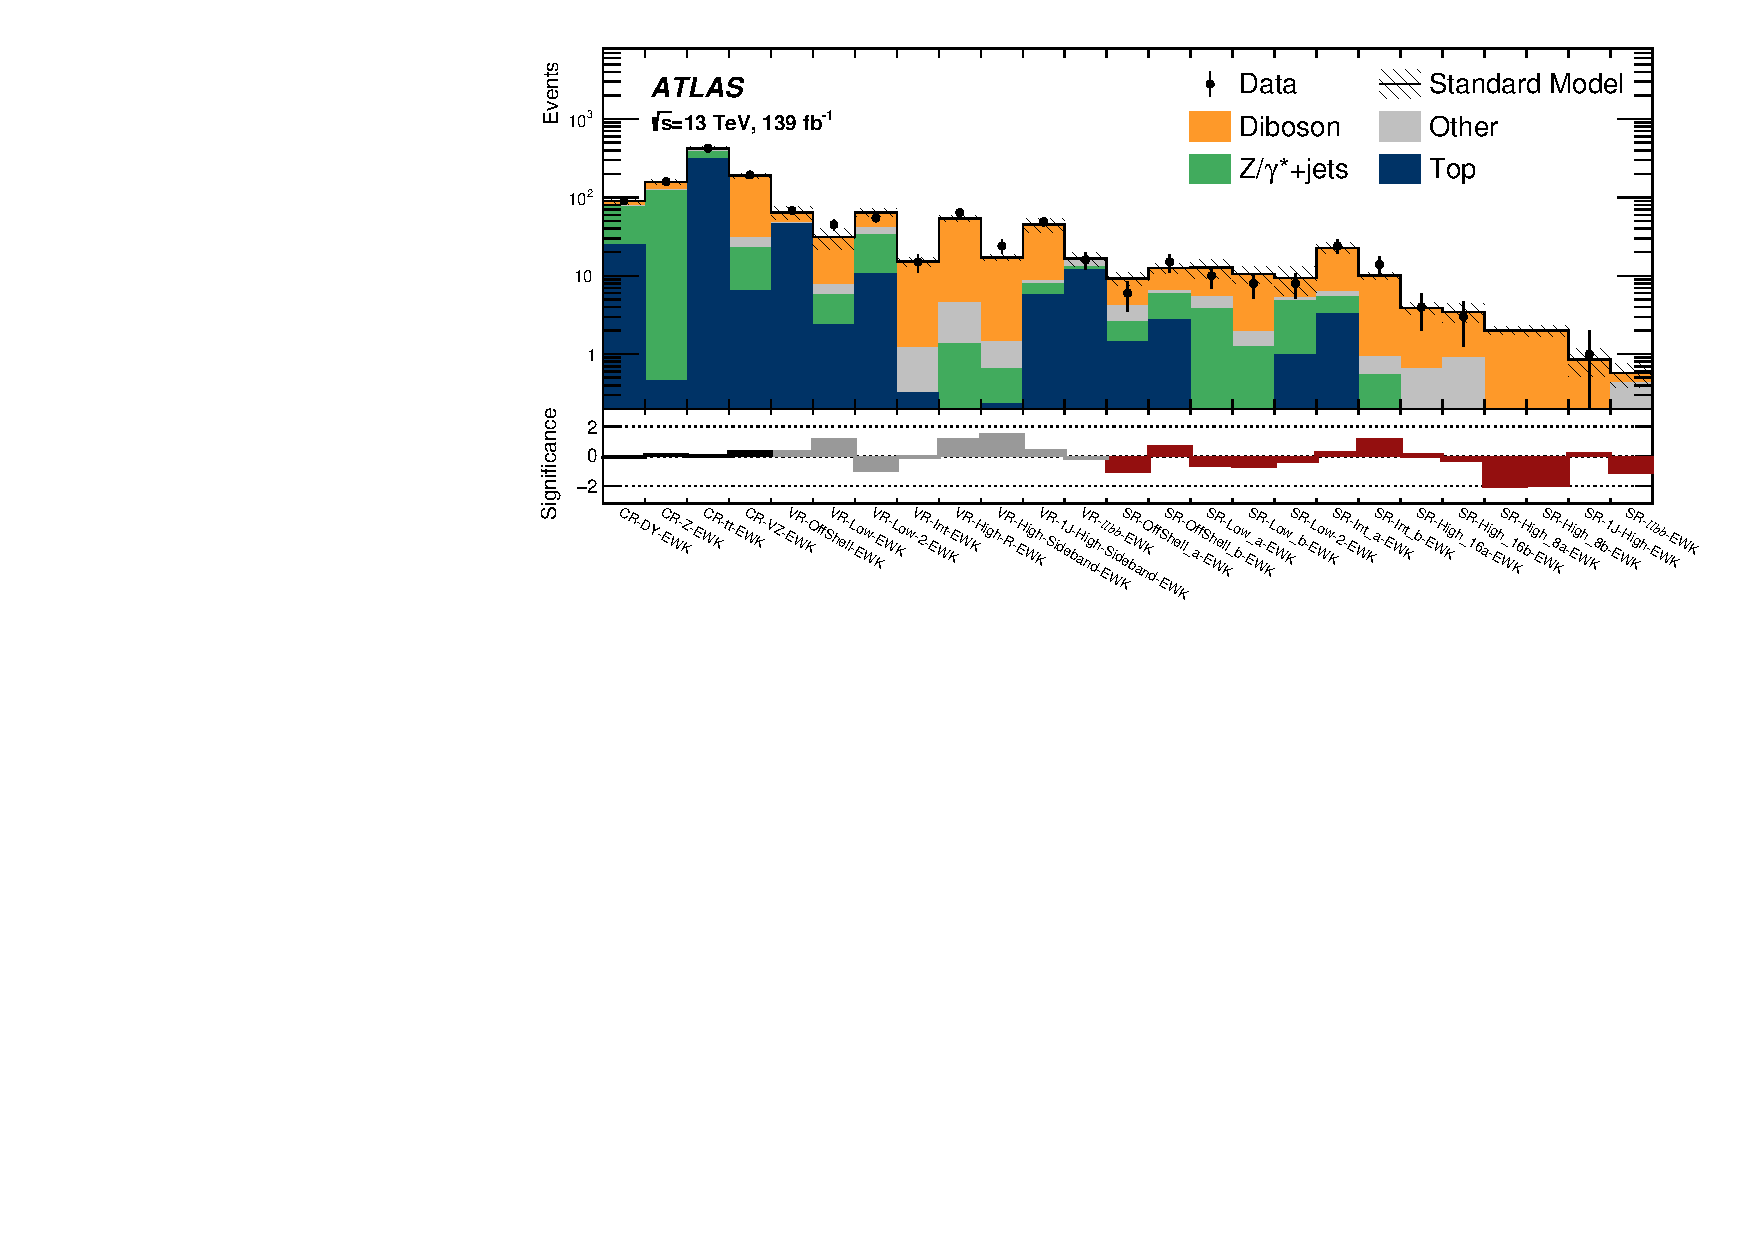
\includegraphics[width=\textwidth]{figures/2ljets_summary_log.pdf}
\caption{%
Data of the $\twoljets$ electroweak analysis with \emph{post-fit}
backgrounds~\cite{atlas2022searches}.
The lower panel shows $S_\mathrm{ATLAS}$ from
Equation~\ref{eqn:significance_atlas}.
Control, validation and signal regions are shown from left to right, with the
regions within each category ordered approximately by their typical $\met$.
Likelihoods from validation regions are not included in the fit.
The `Top' category contains $t\bar t$ and $tW$ processes, and
`Other' contains fake/non-prompt lepton, higgs, triboson, $t\bar tZ$, and other
rare top processes.%
}
\label{fig:2ljets_summary}
\end{figure}


% signal diagrams

\begin{figure}[t]
\centering
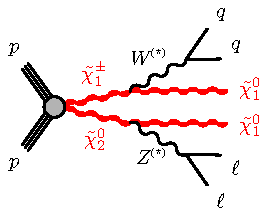
\includegraphics[width=0.48\textwidth]{figures/2ljets_c1n2_llqqn1n1_wz.pdf}
\hfill
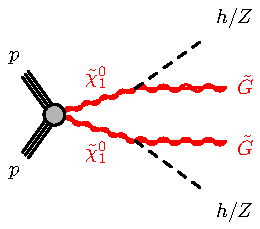
\includegraphics[width=0.45\textwidth]{figures/2ljets_n1n1_hhggzz.pdf}
\caption{%
Supersymmetric signal processes in the $\twoljets$ electroweak
analysis~\cite{atlas2022searches}.
\\[0.5em]
Left: C1N2, where the initial $\chargino_1\textrm{--}\neutralino_2$ pair
is produced through a $s$-channel $W^{\pm}$ resonance and the masses of
weak bosons in decays are bounded by the mass splitting
$m(\chargino_1, \neutralino_2) - m(\neutralino_1)$.
We explore the parameters
$m(\chargino_1, \neutralino_2)$ and $m(\neutralino_1)$.
\\[0.5em]
Right: GMSB, where the initial $\neutralino_1\textrm{--}\neutralino_1$ pair
is produced by soft decays from pairs including $\chargino_1$,
$\neutralino_2$ or $\neutralino_1$.
Although the $h$ and $Z$ bosons decay to many states, we target
$Z\rightarrow \ell\ell$ with
$h/Z\rightarrow bb/jj$.
We explore the parameters
$m(\neutralino_1)$ and $B(\neutralino_1 \rightarrow h \tilde{G})$ with fixed
$m(\chargino_1, \neutralino_2) - m(\neutralino_1) = 1~\eV[G]$.
}
\label{fig:2ljets_signal_diagrams}
\end{figure}


% signal region plots

\begin{figure}[tp]
\centering
\begin{subfigure}{0.49\textwidth}
    \centering
    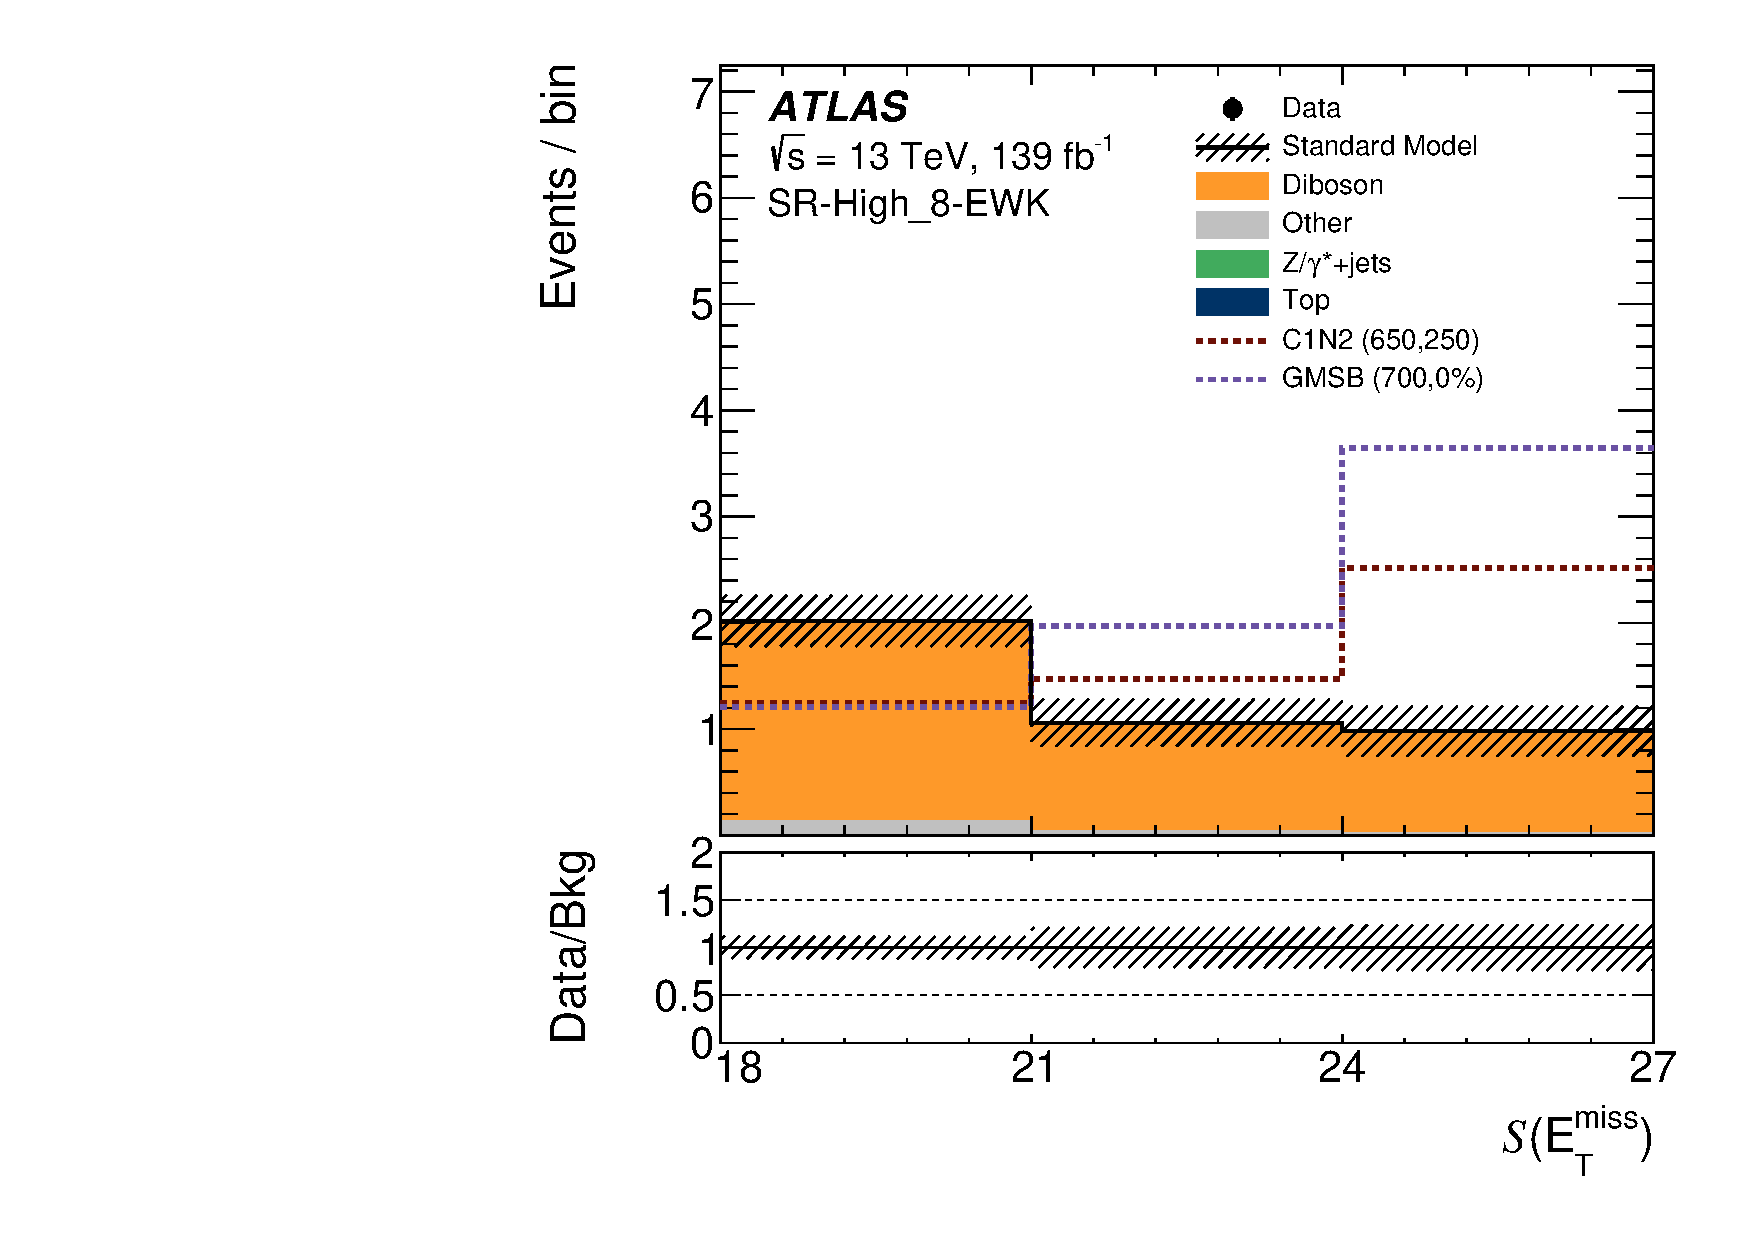
\includegraphics[width=\textwidth]{figures/2ljets_sr_high_8_met_sig.pdf}
    \caption{SR-High-8}
\end{subfigure}
\hfill
\begin{subfigure}{0.49\textwidth}
    \centering
    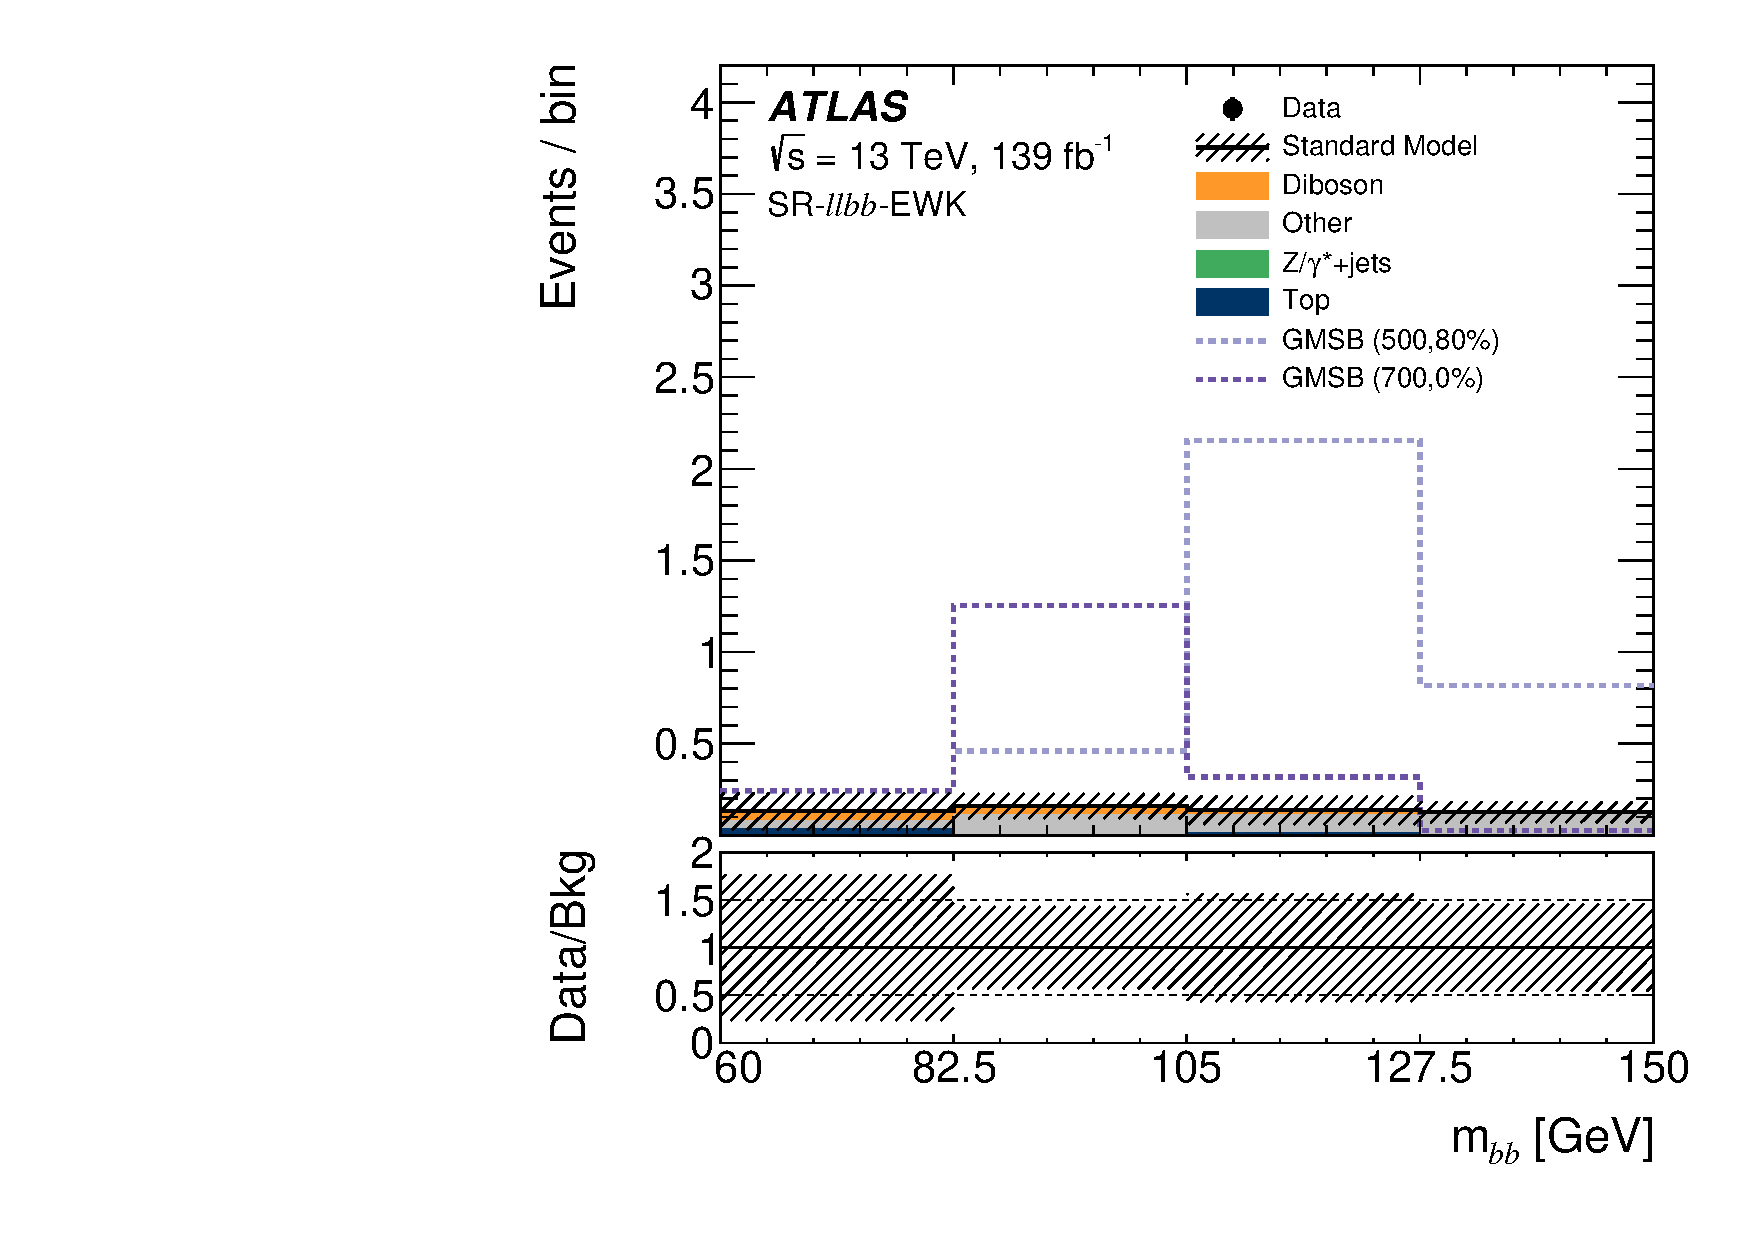
\includegraphics[width=\textwidth]{figures/2ljets_sr_llbb_mbb.pdf}
    \caption{SR-$\ell\ell bb$}
\end{subfigure}
\\[0.5em]
\begin{subfigure}{0.49\textwidth}
    \centering
    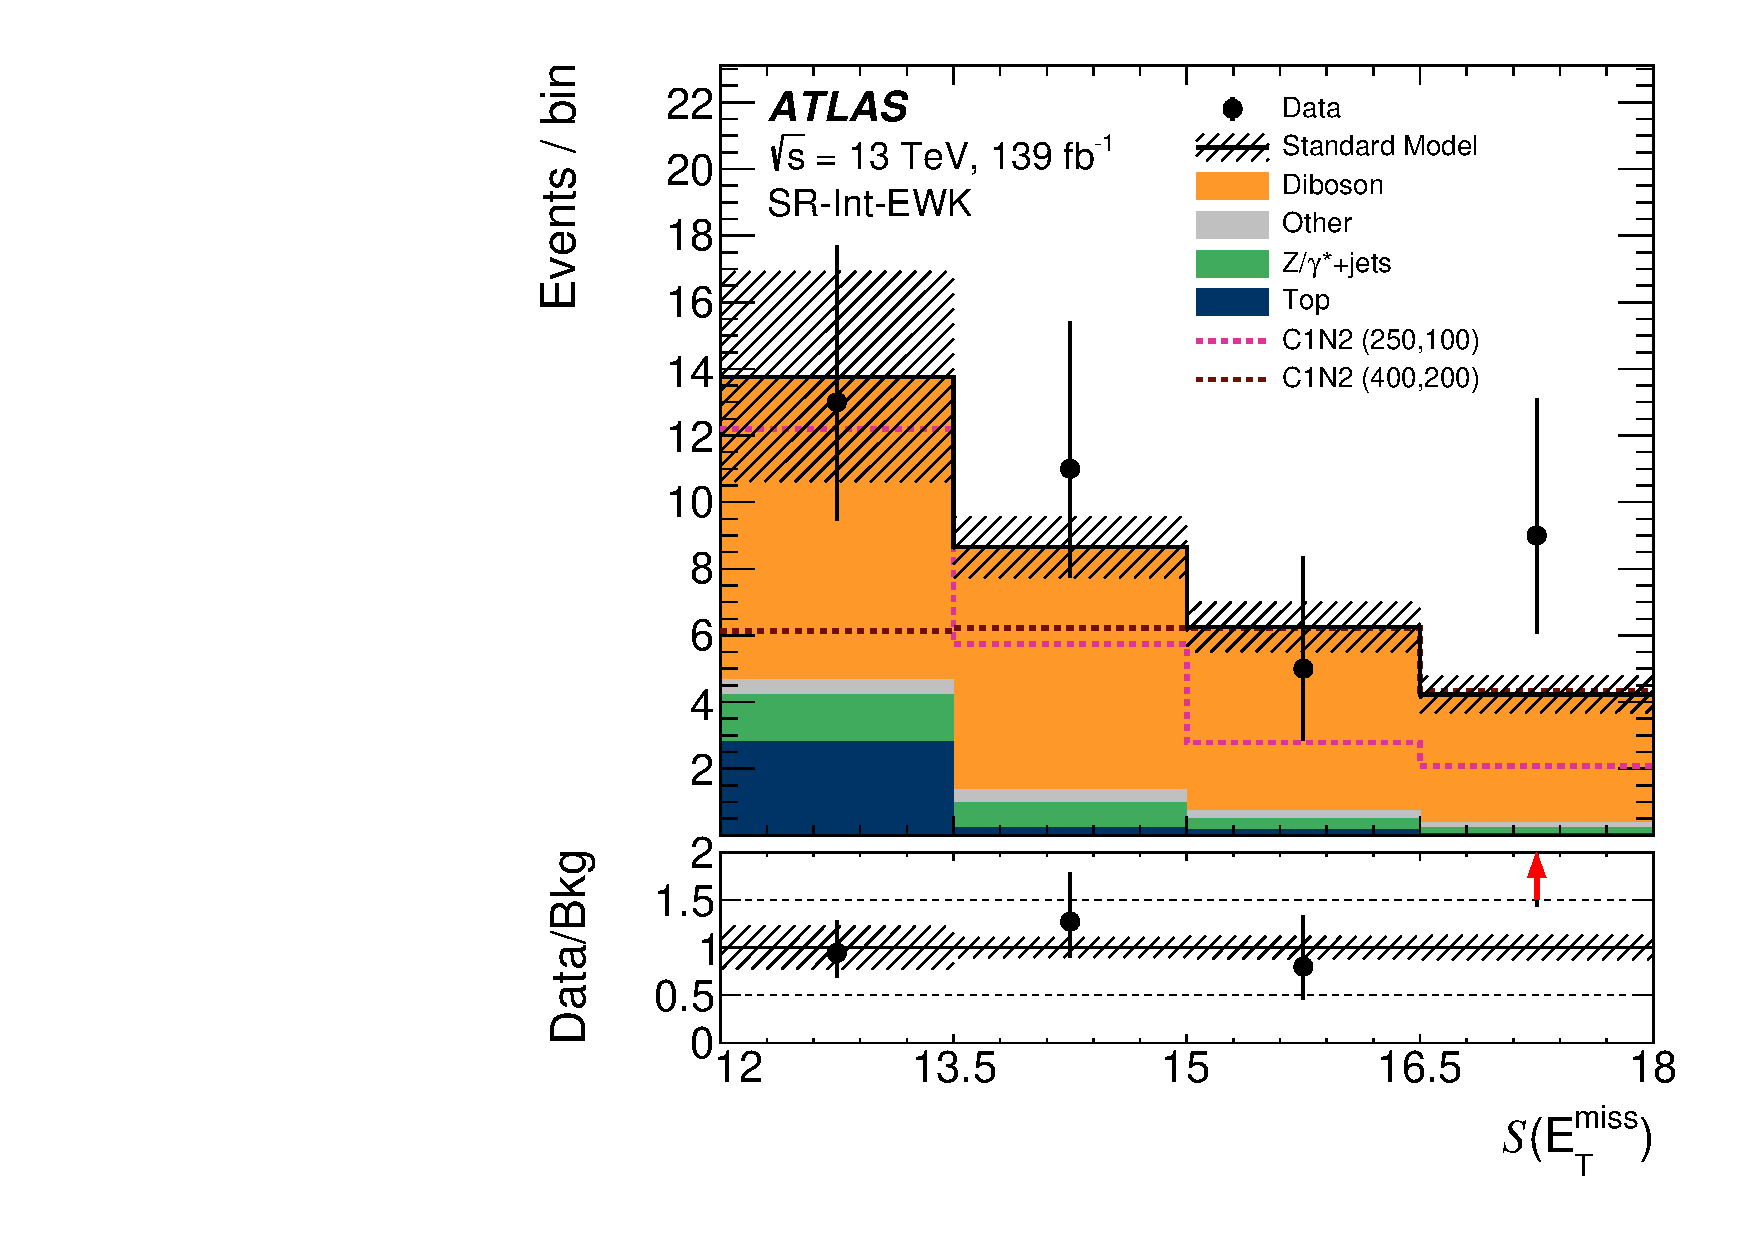
\includegraphics[width=\textwidth]{figures/2ljets_sr_int_met_sig.pdf}
    \caption{SR-Int}
\end{subfigure}
\hfill
\begin{subfigure}{0.49\textwidth}
    \centering
    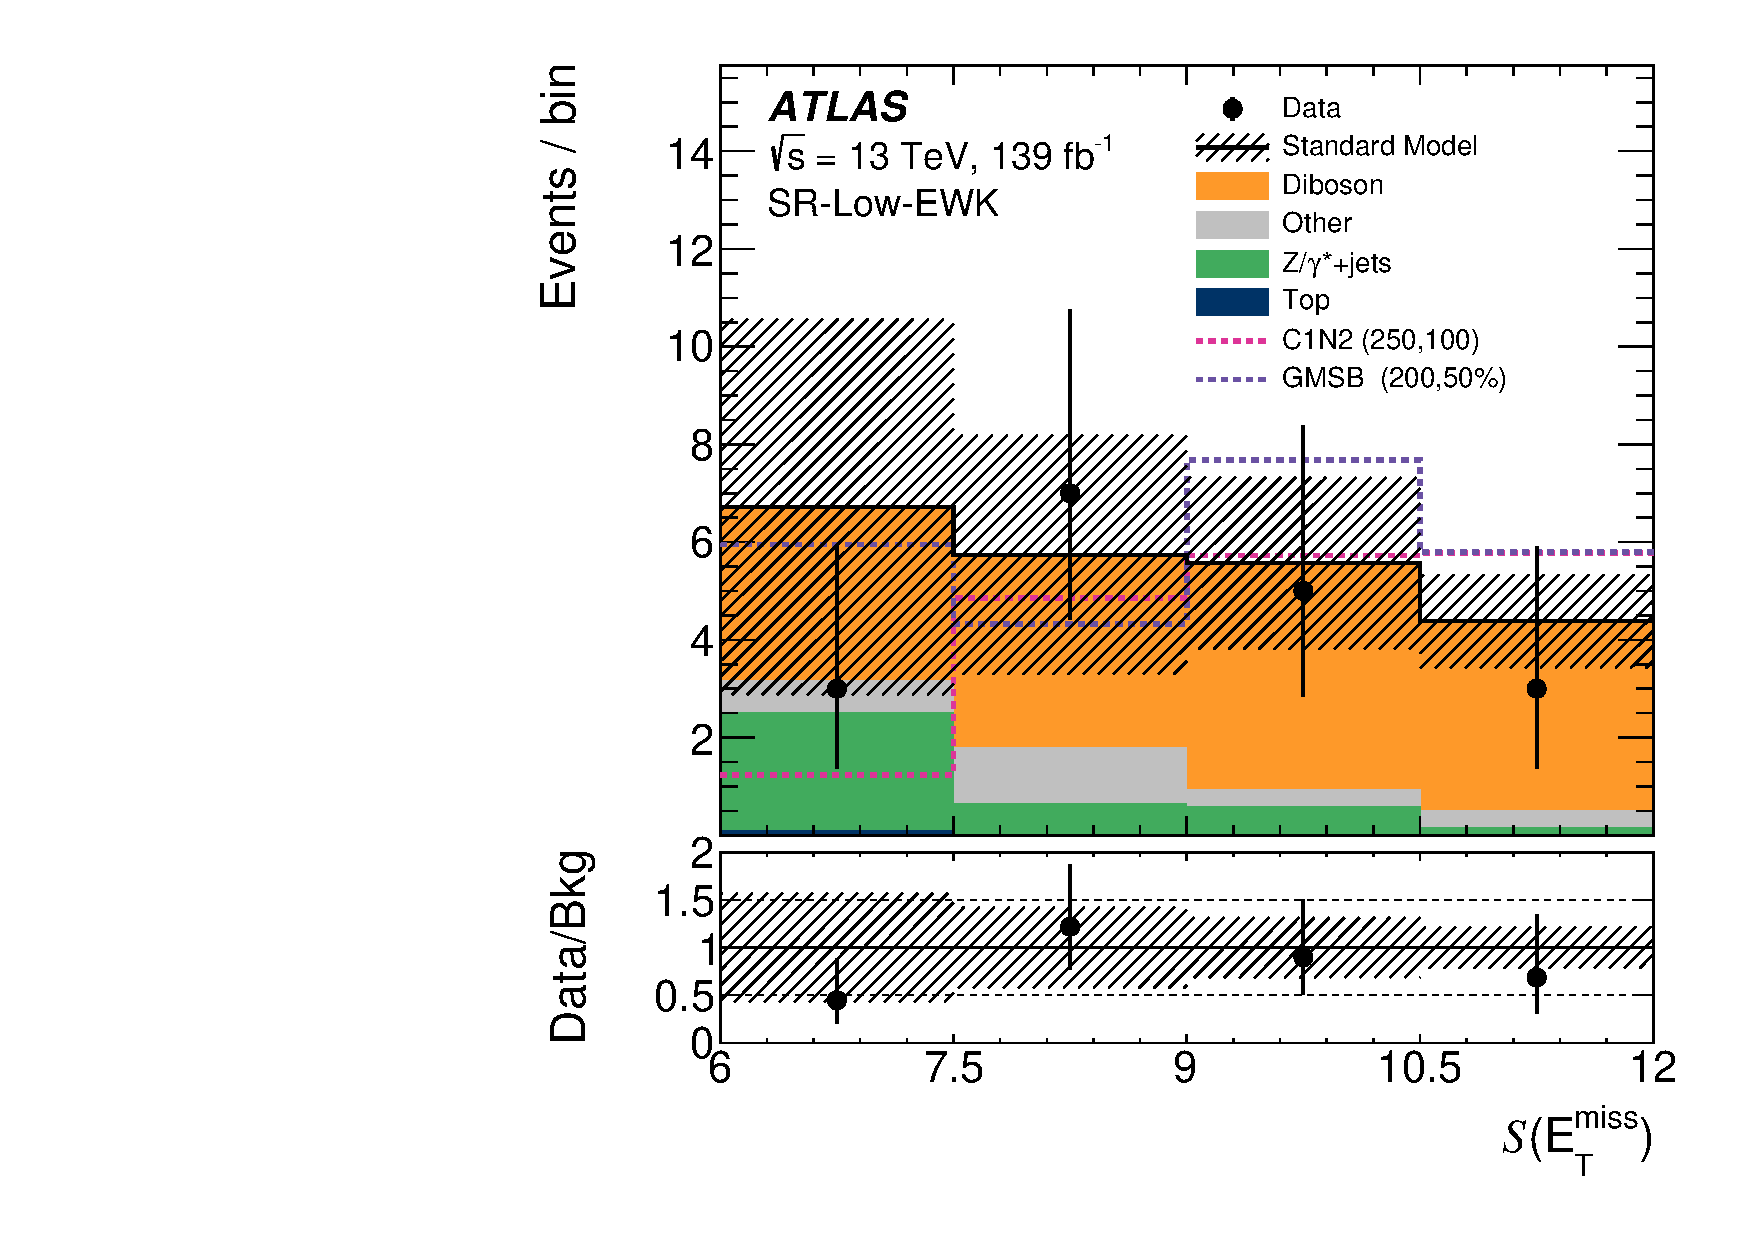
\includegraphics[width=\textwidth]{figures/2ljets_sr_low_met_sig.pdf}
    \caption{SR-Low}
\end{subfigure}
\caption{%
Example signal region histograms with benchmark signal sample yields overlaid
as dotted lines~\cite{atlas2022searches}.
Physically, signal yields would add on top of the backgrounds.
Data are shown; regions in the the top two plots observe zero data, and
Poisson error bars for $0$ events are hidden for aesthetic reasons.
}
\label{fig:2ljets_signal_examples}
\end{figure}


% exclusion plots

\begin{figure}[tp]
\centering
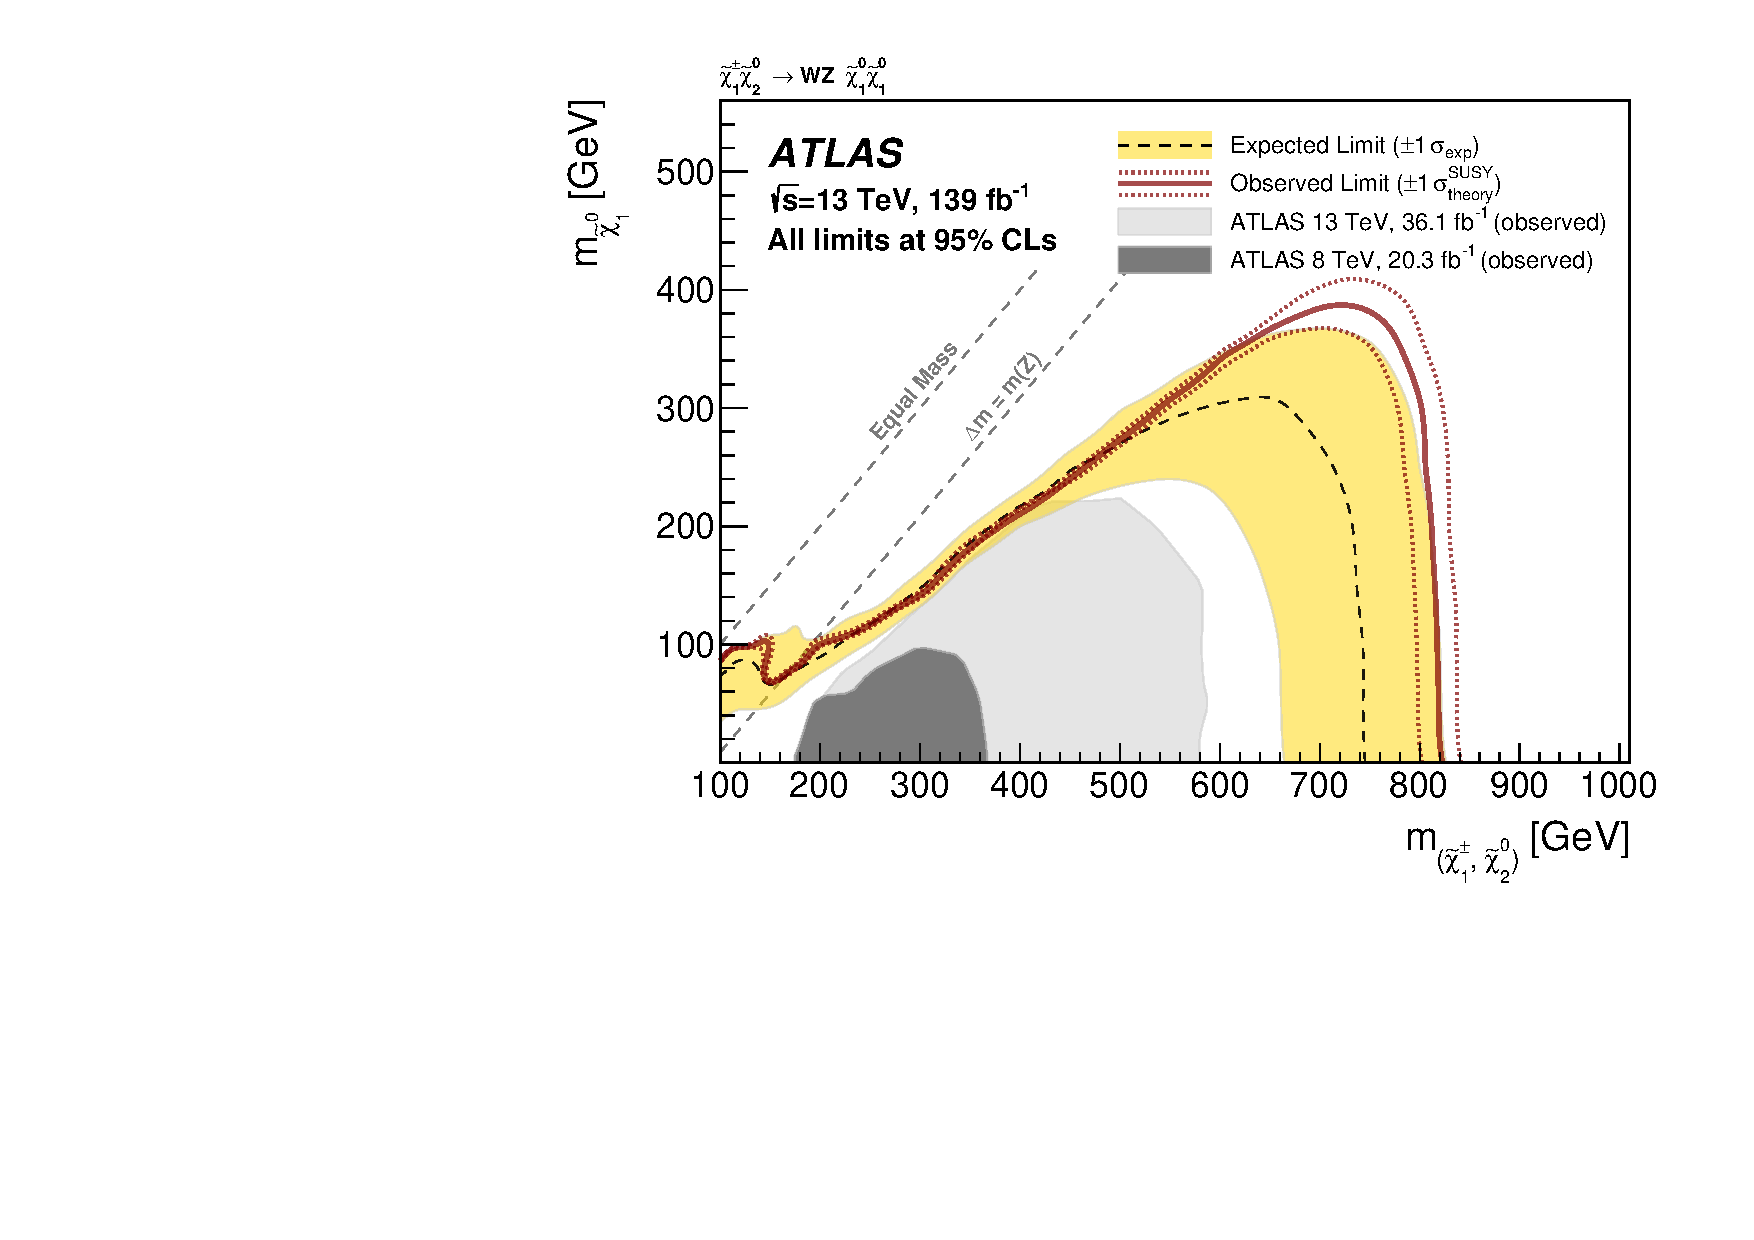
\includegraphics[width=0.99\textwidth]{figures/2ljets_contours_c1n2.pdf}
\caption{%
Contours for the C1N2 model in the $\twoljets$ electroweak
analysis~\cite{atlas2022searches}.
\\[0.5em]
Space below the solid red line is labelled as excluded and its dotted
neighbours show the result if all signal cross-sections are varied up and down
by theoretical error bars.
\\[0.5em]
The yellow band shows the $\pm1$-sigma region of exclusion contours
from asymptotic approximations to the prior distribution of the test statistic.
Grey areas are observed limits from the two-lepton parts
of~\cite{atlas_23l_SUSY_2016_24} and~\cite{atlas_2l_SUSY_2013_11}.
Exclusion is defined by the $95\%$ $\mathrm{CLs}$ prescription
in asymptotic approximations.
All contours are interpolated from a sparse grid.
}
\label{fig:2ljets_contours_c1n2}
\end{figure}

\begin{figure}[tp]
\centering
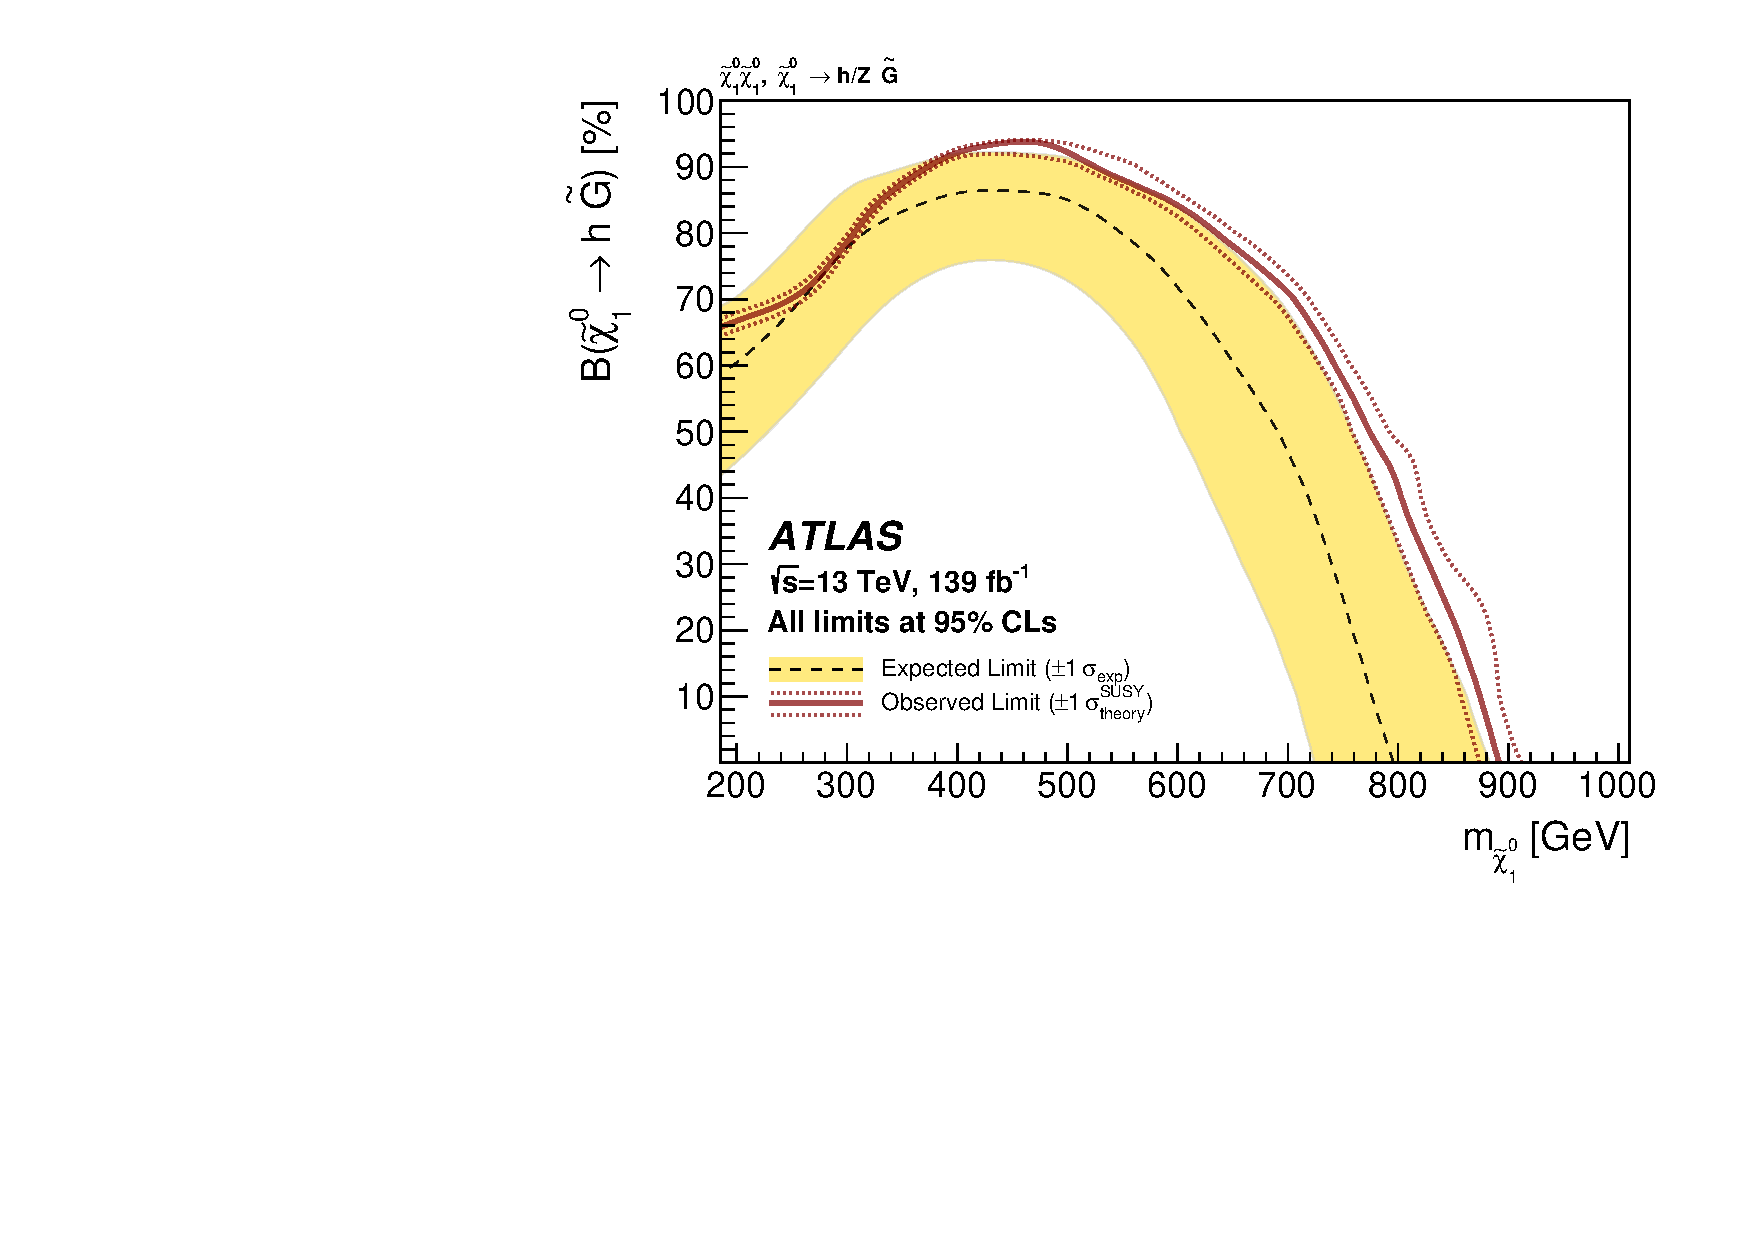
\includegraphics[width=0.99\textwidth]{figures/2ljets_contours_gmsb.pdf}
\caption{%
Contours for the GMSB model in the $\twoljets$ electroweak
analysis~\cite{atlas2022searches}.
\\[0.5em]
Space below the solid red line is labelled as excluded and its dotted
neighbours show the result if all signal cross-sections are varied up and down
by theoretical error bars.
\\[0.5em]
The yellow band shows the $\pm1$-sigma region of exclusion contours
from asymptotic approximations to the prior distribution of the test statistic.
Exclusion is defined by the $95\%$ $\mathrm{CLs}$ prescription
in asymptotic approximations.
All contours are interpolated from a sparse grid.
}
\label{fig:2ljets_contours_gmsb}
\end{figure}


% upper limits
% definitely want this after pictures
\FloatBarrier
\begin{table}[tp]
\centering
% custom separator for aligned +-
% https://stackoverflow.com/a/2132998
\begin{tabular*}{\textwidth}{lr@{$~\pm~$}lccrrcc}
Region &
\multicolumn{2}{c}{Fitted} &
Data &
$\langle A\epsilon{ \sigma}\rangle_{\mathrm{obs}}^{95}~\mathrm{fb}$ &
$S_{\mathrm{obs}}^{95}$  &
$S_{\mathrm{exp}}^{95}$ &
$\mathrm{CLb}$ &
$p(s=0)$  \\[1.5ex]
DR-OffShell      & $22.1$ & $2.7$ & 21 & $0.10$ & $14.3$ & $12.3^{+4.7}_{-3.1}$ & $0.68$ & $0.50$ \\[.5ex]
DR-Low           & $22$ & $4$ & 18 & $0.08$ & $10.8$ & $15.3^{+5.7}_{-4.0}$ & $0.09$ & $0.50$ \\[.5ex]
DR-Int           & $35$ & $4$ & 38 & $0.15$ & $20.9$ & $17.5^{+5.9}_{-3.9}$ & $0.73$ & $0.23$ \\[.5ex]
DR-High          & $3.9$ & $0.5$  & 0  & $0.02$ & $3.0$ & $5.6^{+2.2}_{-1.5}$ & $0.00$ & $0.50$ \\[.5ex]
DR-$\ell\ell bb$ & $0.51$ & $0.20$  & 0  & $0.02$ & $3.0$ & $3.0^{+1.3}_{-0.0}$ & $0.19$ & $0.50$ \\[.5ex]
\end{tabular*}
\caption{%
Upper limit results in $\twoljets$ electroweak discovery
regions~\cite{atlas2022searches}.
The fitted yield is in the background-only model constrained by the data in each region.
Limits are intended to reflect constrains on additive signal contributions.
\\[0.5em]
Left to right:
the region name,
the post-fit background expectation,
the number of data observed,
the observed $95\%$ $\mathrm{CLs}$ upper limit on the visible cross-section
$\langle\epsilon\sigma\rangle_\mathrm{obs}^{95}$,
its corresponding signal expectation $S_\mathrm{obs}^{95}$,
the expected $95\%$ upper limits on the signal expectation $S_\mathrm{exp}^{95}$
as would be obtained were the test statistic given by its central or
$\pm1$-sigma variations,
$\mathrm{CLb}$ evaluated with the signal expectation set to the observed upper limit,
and the discovery $p$-value (capped at $0.5$) with its equivalent significance.
\\[0.5em]
Upper limits use the one-sided profile likelihood test statistic.
The discovery $p$-value uses a profile likelihood test statistic in a one-sided test.
All $p$-values are estimated by simulation of alternative data.
\TODO{add labels and references to asymptotic formulae paper}
\TODO{reference pdg rounding}
}
\label{tab:2ljets_discovery}
\end{table}

\FloatBarrier
\subsection{Contributions}

In this subsection, I claims attributions of work on the $\twoljets$ analysis
and related \atlas\ efforts.

\begin{itemize}
\item Design, implementation and execution of the electroweak part of the analysis.
\item Service as `analysis contact' from January to October 2020.
\item Production of main data inputs for all three $\twoljets$ analyses
and the RJR $3\ell$ search~\cite{atlas_rjr_3l_SUSY_2019_09},
Production of all systematic variations for the background samples;
other group members assisted with the central background sample.
Production of all electroweak signal samples and their systematic variations.
\item \TODO{?Evaluation of Monte Carlo $Z$+jets uncertainties for RJR signal regions
which indicated they exceeded $100\%$}
\item \TODO{Various collaborations with group members on scripts to conduct
tasks which were common between the searches.}
\item Integration of the electroweak analysis with ATLAS combinations and
pMSSM scan efforts, by performing their validation studies and serializing the
analysis results.
\item Preparation of electroweak results for publication in the
paper~\cite{atlas2022searches} and the public HEPData
record~\cite{maguire2017hepdata}.
\end{itemize}
Except where specified, I produced all figures presented in this thesis.
Many plotting scripts, however, are modified from versions inherited from
many \atlas\ members past and present to whom I am grateful.

Of the large collaboration involved in this project, a great deal of credit is
due to the following colleagues, labelled with their primary focus within
the $\twoljets$ search effort:
Knut Oddvar Vadla (electroweak),
Sarah Williams (electroweak),
Jason Lea Oliver (RJR),
Abhishek Sharma (RJR),
Jonathan Long (strong),
Arka Santra (strong),
Matt Zhang (strong),
Yumeng Cao (various),
Eirik Gramstad (fake/non-prompt leptons),
Benjamin Henry Hooberman (leadership).
Cheers.

\clearpage
\FloatBarrier
\section{Context}
\label{sec:2ljets_context}
% previous results on 2(/3)L from ATLAS
% other constraints on these models from ATLAS/CMS
% previous region design, motivation for this work
Previous analyses of \atlas\ data have explored similar selections of
two leptons, jets, and missing transverse momentum.
Quite a few analyses, in fact.
This project exists to supplement those results with information from the full
LHC Run 2 data-set which was completed in 2018 and contains
$139~\mathrm{fb}^{-1}$ of usable proton-proton collisions at $\sqrt{s} = 13~\eV[T]$.
Leverage of the increased data quantity is one key aim.
Analysis quality also might be improved if our designs can take lessons from
the experiences of previous work.

% electroweak
% Run 1 data~\cite{atlas_2l_SUSY_2013_11},
% partial Run 2 data~\cite{atlas_23l_SUSY_2016_24},
% atlas_rjr_23l_SUSY_2017_03,
% atlas_rjr_mimic_SUSY_2018_06

The $\twoljets$ analysis is a trinity,
of which all three parts update previously published \atlas\ results.
These three parts are named `RJR', `electroweak', and `strong', each of which
is described in its historical context in this section.

Recursive Jigsaw Reconstruction (RJR) is an algorithm for constructing useful
event variables.
The $\twoljets$ RJR analysis, detailed in Section~\ref{sec:2ljets_origins_rjr},
uses RJR variables to define its regions in a signal-independent search.

My primary contributions are to the $\twoljets$ electroweak analysis,
detailed in Section~\ref{sec:2ljets_origins_electroweak},
which uses conventional (non-RJR) event variables to define a collection of
orthogonal regions, and performs a search for effects from the electroweak
sectors of supersymmetric models.

Unsurprisingly, the strong part of the $\twoljets$ analysis is
detailed in Section~\ref{sec:2ljets_origins_strong} and
searches for effects from the strong sector.
It also uses conventional event variables, and focuses on features in the
distribution of the invariant masses of lepton pairs.


\subsection{RJR}
\label{sec:2ljets_origins_rjr}

\begin{figure}[tp]
\centering
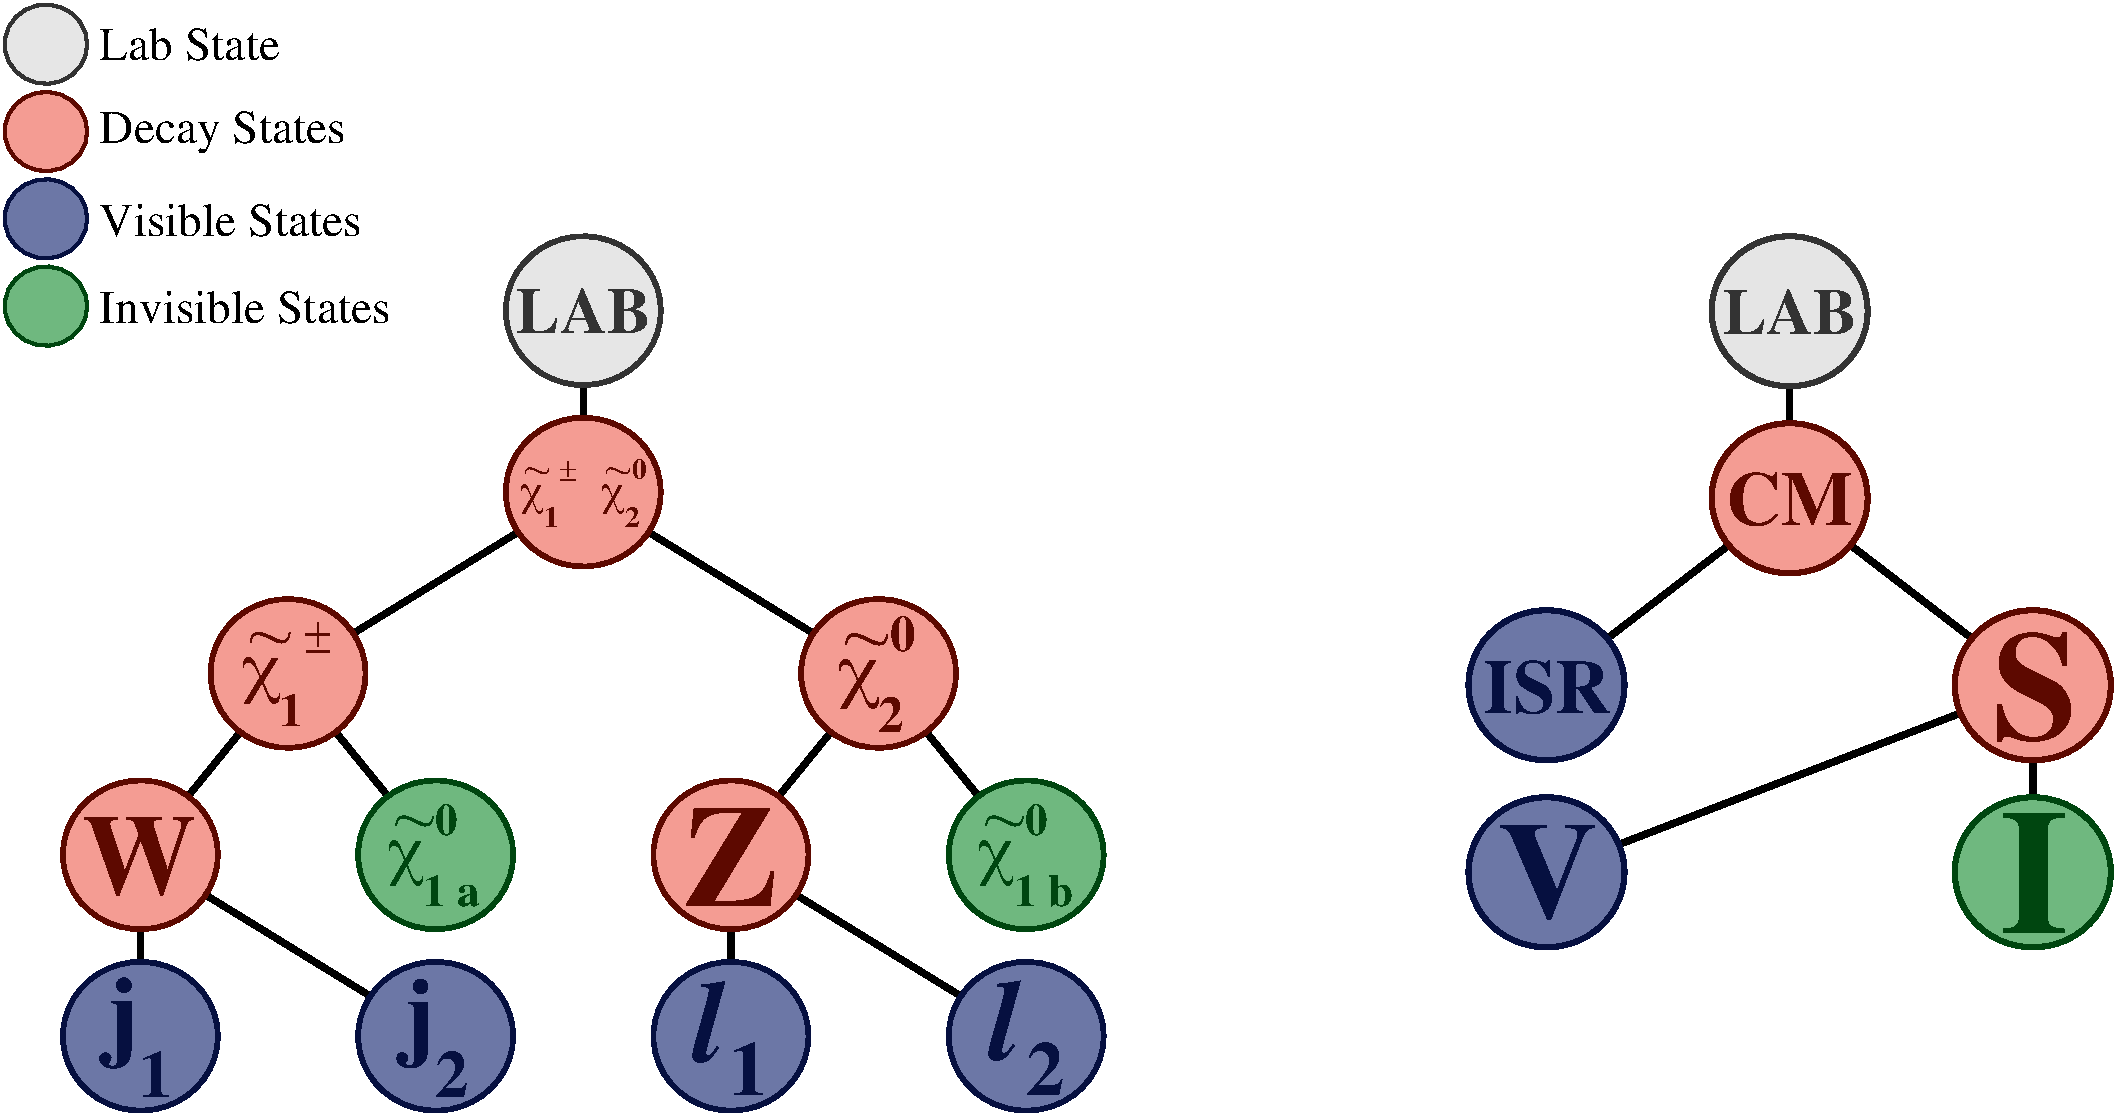
\includegraphics[width=0.9\textwidth]{figures/2ljets_rjr_trees.pdf}
\caption{%
Decay trees for the $\twoljets$ RJR analysis~\cite{atlas2022searches}.
Both diagrams represent processes also targetted in the electroweak analysis.
(left) A fully-resolved decay tree with its particles labelled.
(right) Only the $Z\rightarrow\ell\ell$ (\underline{V}ector boson)
is resolved, but the supersymmetric system recoils off
hard QCD jets labelled ``ISR'', boosting the \underline{I}nvisible particles,
to generate visibly large $\met$ in models with small mass-splittings.
The same approach is used for SR-OffShell selections in the electroweak
analysis.
\emph{This figure was made by the RJR team.}
}
\label{fig:2ljets_rjr_decay_trees}
\end{figure}

The Recursive Jigsaw Reconstruction (RJR) method interprets reconstructed
particle data by reconciling them with user-specified decay trees, and works
by making decisions of how to assign four-momenta to different `systems',
which are nodes of the chosen the decay graph.
Event variables are then evaluated in those systems' rest
frames~\cite{jackson2017sparticles, jackson2017rjr}.

In this way, RJR variables get some intelligence in how parent particles are
reconstructed from their visible decay products, as well as approximate
independence from uninteresting boosts, particularly those from the emission of
QCD jets outside of the supersymmetric decay tree.

Over the last several years, RJR event variables have been demonstrated to be
effective for interpreting supersymmetric particle physics
data~\cite{santoni2018probing},
and have been used in numerous \atlas\ searches~\cite{%
atlas_rjr_SUSY_2016_07,
atlas_rjr_SUSY_2016_15,
atlas_rjr_SUSY_2016_16,
atlas_rjr_23l_SUSY_2017_03,
atlas_rjr_SUSY_2018_12,
atlas_rjr_EXOT_2019_19,
atlas_rjr_3l_SUSY_2019_09
}.
They have also influenced the designs of other analyses which do not use
RJR variables themselves~\cite{atlas_rjr_mimic_SUSY_2018_06}.


Two decay trees are used in the $\twoljets$ RJR analysis, with signal region
each.
These trees target C1N2-like scenarios similar to those also considered in the
$\twoljets$ electroweak search,
and illustrated in Figure~\ref{fig:2ljets_rjr_decay_trees}.

\subsubsection{Former excesses}
Excess data were observed in several signal regions of the partial Run 2
search ``for chargino--neutralino production using recursive
jigsaw reconstruction in final states with two or three charged
leptons''~\cite{atlas_rjr_23l_SUSY_2017_03},
which used $36.1~\mathrm{fb}^{-1}$ of proton-proton collisions at
$\sqrt{s} = 13~\eV[T]$.
That search reported notable excesses in four signal regions.
Of these, two required two charged leptons
($\mathrm{SR}2\ell\_\mathrm{Low}$ and $\mathrm{SR}2\ell\_\mathrm{ISR}$),
and other two required three
($\mathrm{SR}3\ell\_\mathrm{Low}$ and $\mathrm{SR}3\ell\_\mathrm{ISR}$).

Although the largest local excess was reported as ``$3.0$ standard deviations'',
which is not particularly large, the pattern of four related regions with
excess data can understandably draw attention.

Both $\mathrm{SR}3\ell\_\mathrm{Low}$ and $\mathrm{SR}3\ell\_\mathrm{ISR}$
have been revisited with the full Run 2 data-set and updated background
modelling;
the update sees ``no significant excesses''~\cite{atlas_rjr_3l_SUSY_2019_09}.
These regions have also been approximated without direct use of RJR event
variables;
those approximations also find data ``in agreement'' with the background
model~\cite{atlas_rjr_mimic_SUSY_2018_06}.

The $\twoljets$ RJR serves to analysis reproduce
$\mathrm{SR}2\ell\_\mathrm{Low}$ and $\mathrm{SR}2\ell\_\mathrm{ISR}$,
with the full Run 2 data-set and updated background modelling,
and asks whether the excesses persist.
They do not.


\begin{figure}[tp]
\centering
\begin{subfigure}{0.49\textwidth}
    \centering
    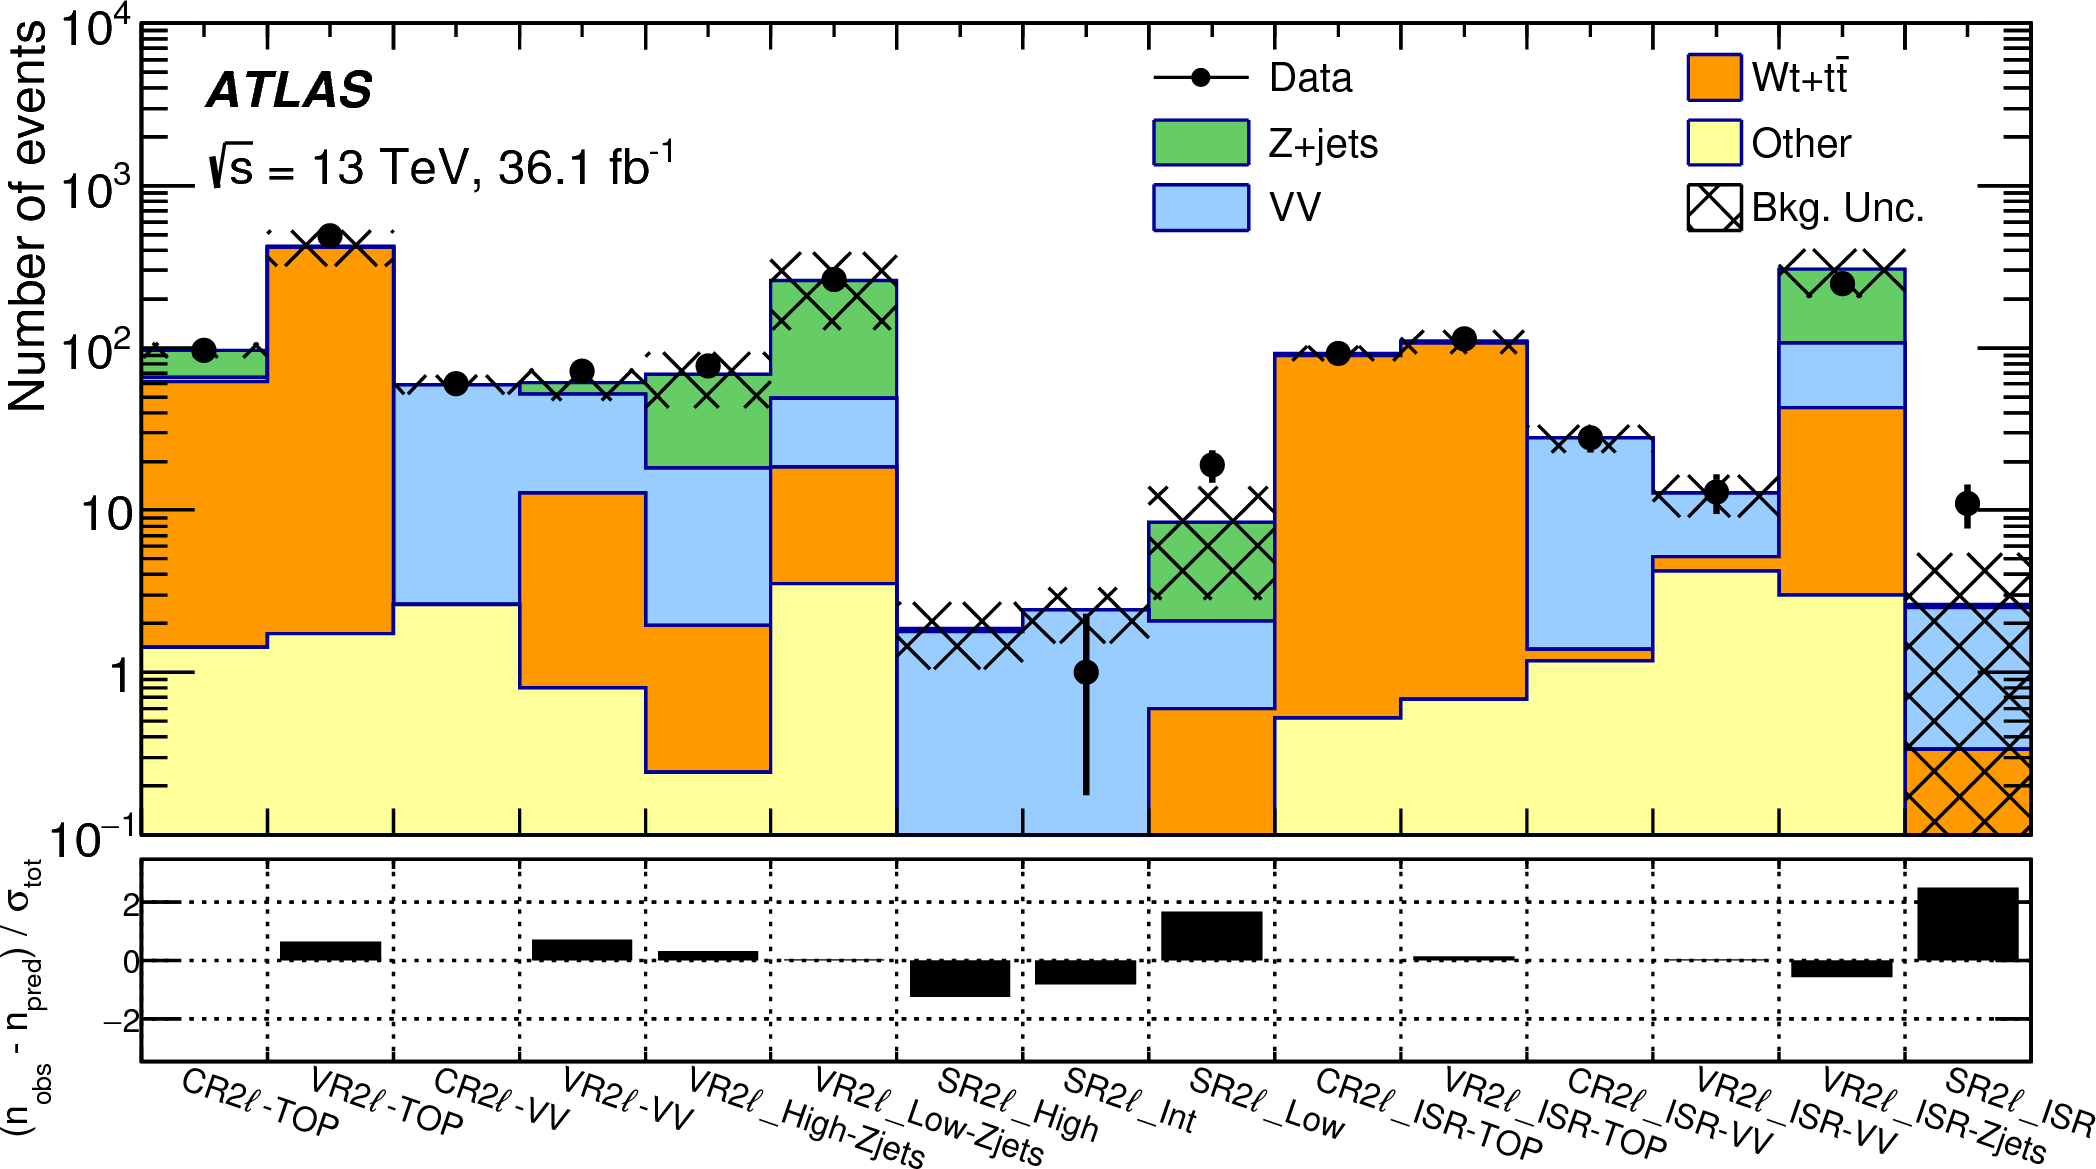
\includegraphics[width=\textwidth]{figures/2ljets_rjr_23l_2l_summary.png}
    \caption{$2\ell$ RJR~\cite{atlas_rjr_23l_SUSY_2017_03}}
\end{subfigure}
\hfill
\begin{subfigure}{0.49\textwidth}
    \centering
    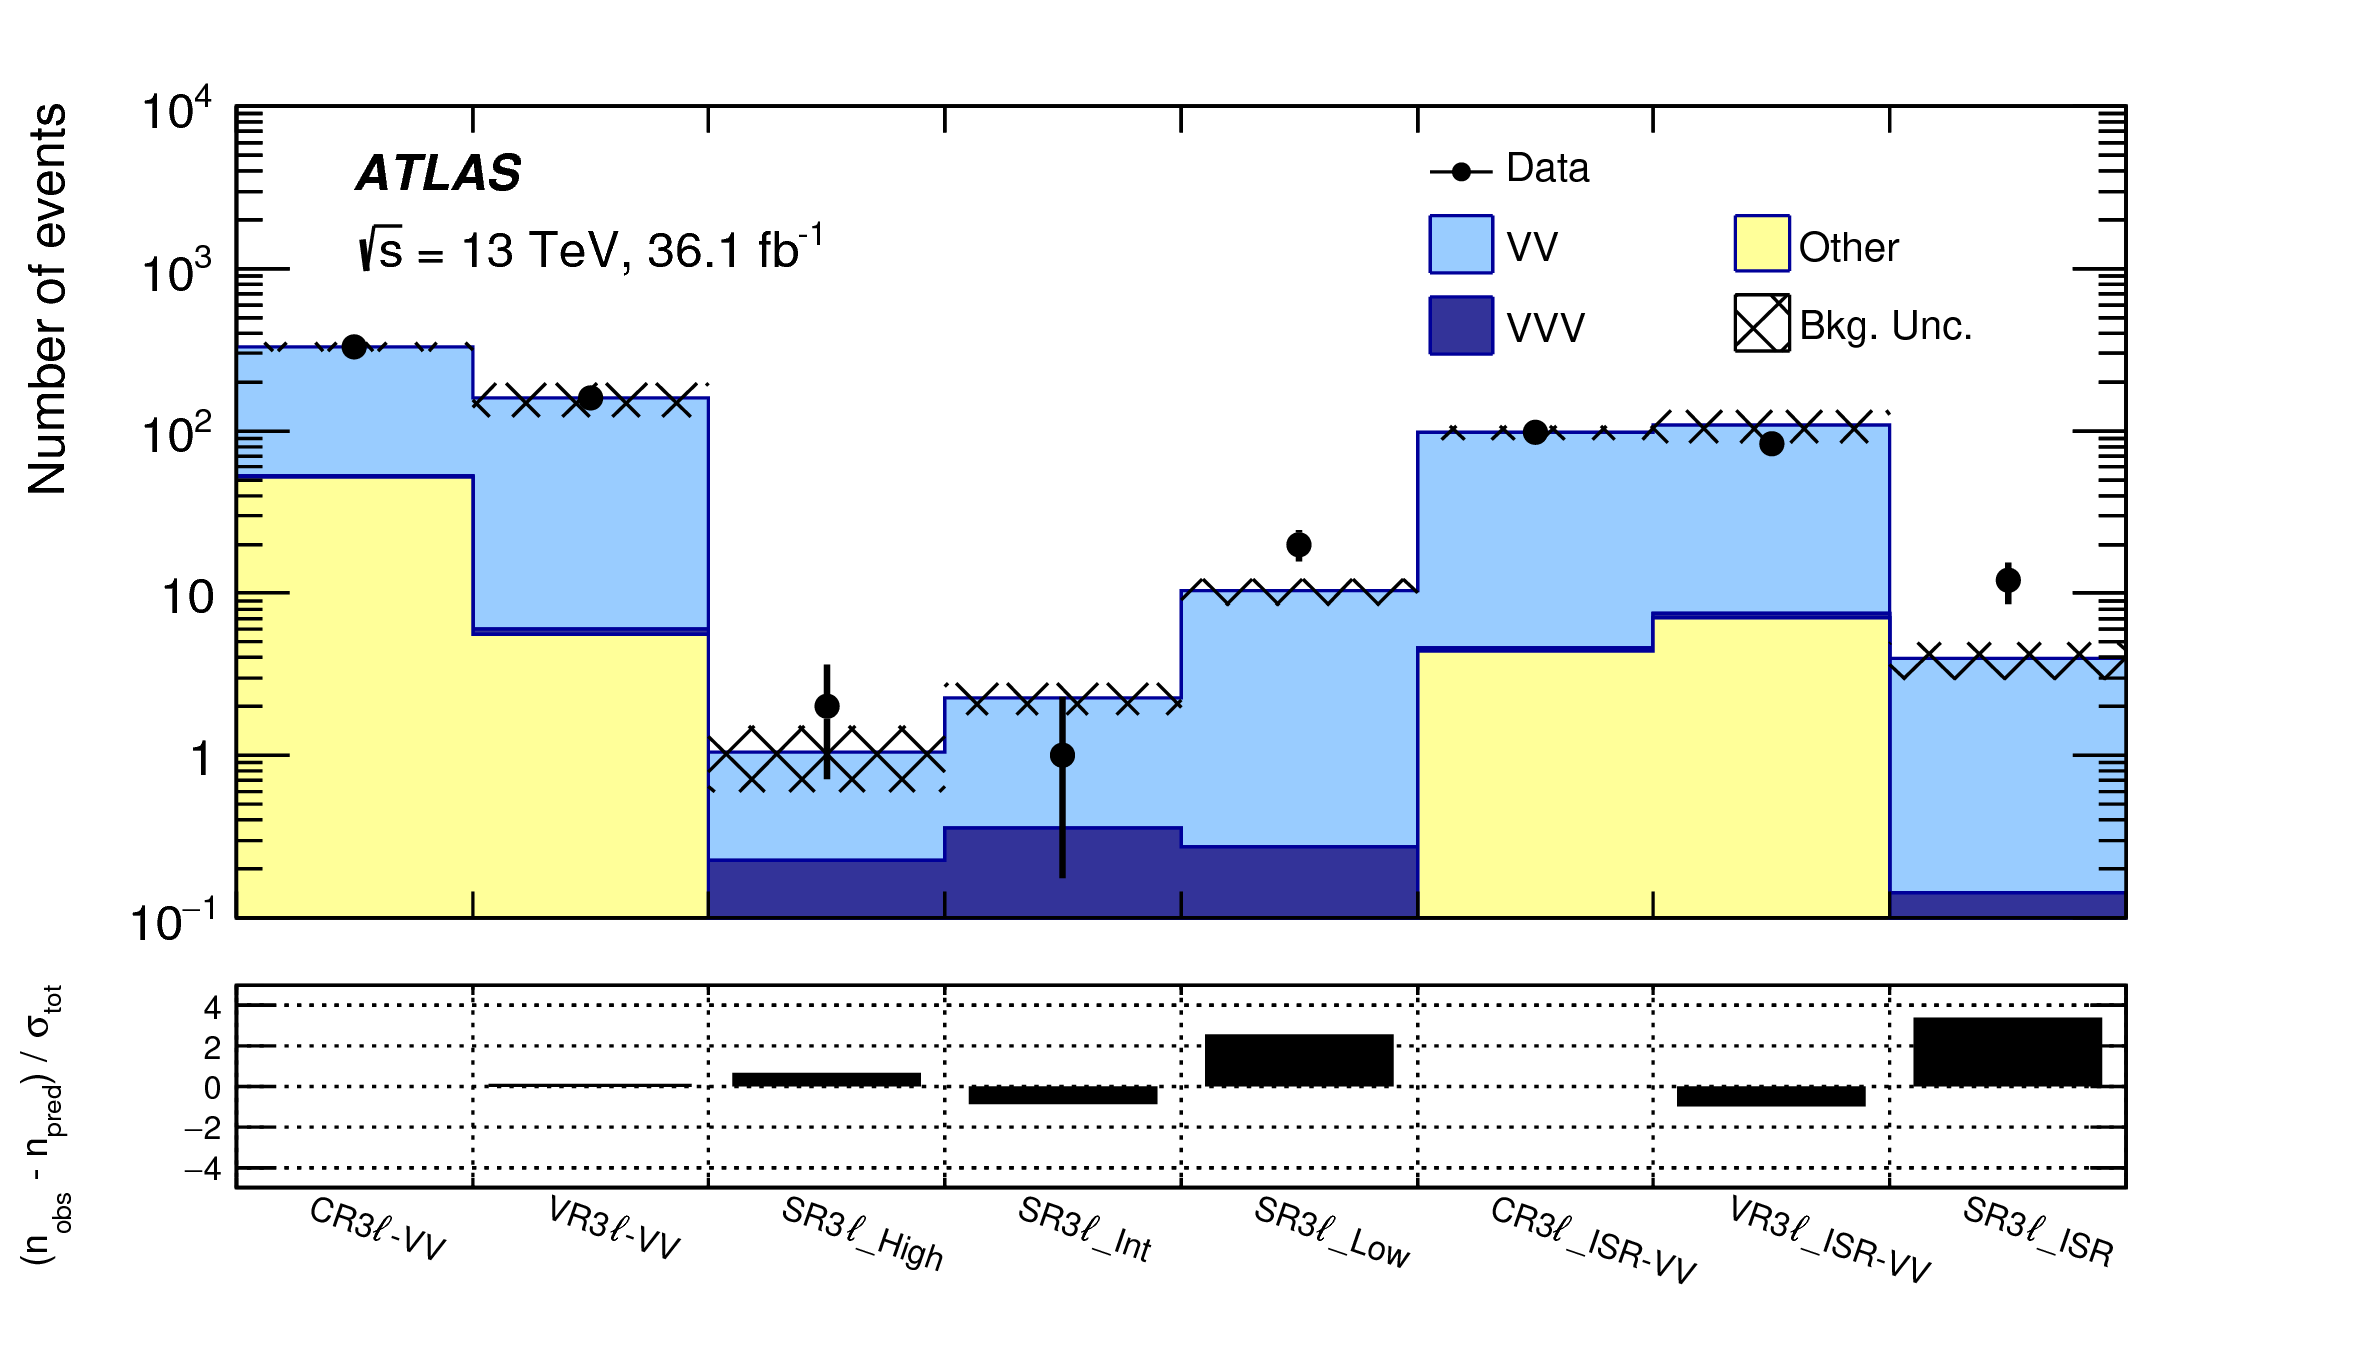
\includegraphics[width=\textwidth]{figures/2ljets_rjr_23l_3l_summary.png}
    \caption{$3\ell$ RJR~\cite{atlas_rjr_23l_SUSY_2017_03}}
\end{subfigure}
\\[0.5em]
\begin{subfigure}{0.8\textwidth}
    \centering
    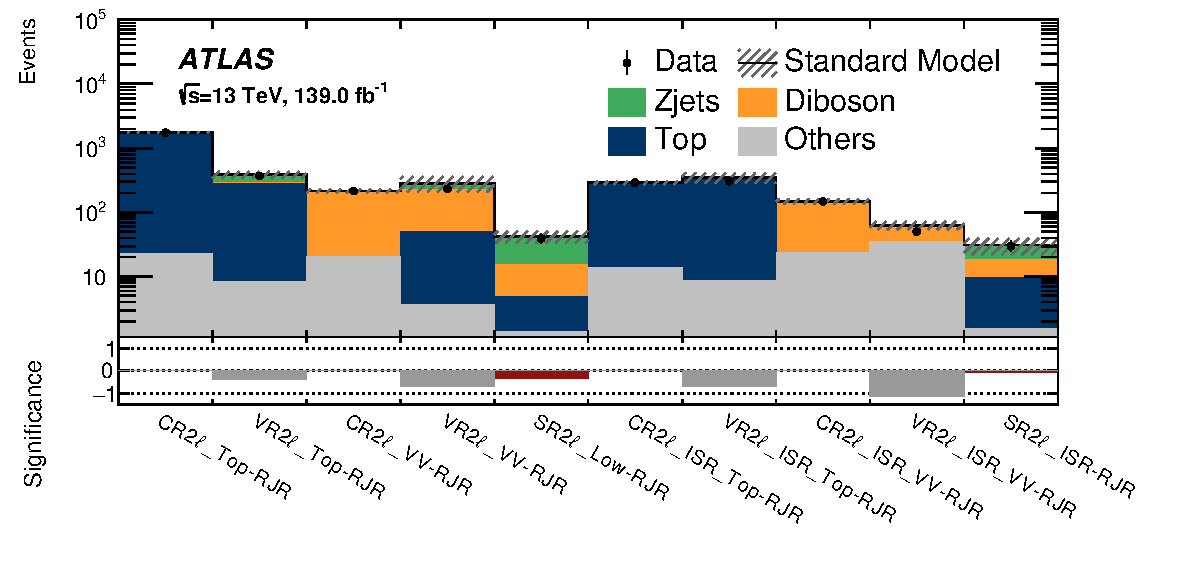
\includegraphics[width=\textwidth]{figures/2ljets_rjr_summary_log.pdf}
    \caption{$\twoljets$ RJR~\cite{atlas2022searches}}
\end{subfigure}
\caption{%
Summary plots for RJR analyses:
(a) and (b)~two- and three- lepton selections respectively reproduced
from~\cite{atlas_rjr_23l_SUSY_2017_03},
(c)~all regions from the $\twoljets$ RJR search~\cite{atlas2022searches}.
Note the excesses in
$\mathrm{SR}2\ell\_\mathrm{Low}$ and $\mathrm{SR}2\ell\_\mathrm{ISR}$ of (a),
and in
$\mathrm{SR}3\ell\_\mathrm{Low}$ and $\mathrm{SR}3\ell\_\mathrm{ISR}$ of (b).
\textit{Sub-figure (c) was made by the RJR team.}
}
\label{fig:2ljets_signal_examples}
\end{figure}


\subsubsection{Doubts}
Disappearing excesses have encouraged some doubts about RJR variables in
certain social circles;
the existence of the `RJR-mimic' paper~\cite{atlas_rjr_mimic_SUSY_2018_06}
is public evidence of this.

A more precisely framed problem with RJR variables is that they tend to select
phase space which is poorly modelled by simulations.
This is plausibly explained by the fact that  RJR variables are non-trivially
related to conventional, lab-frame variables.
Simulations have been tuned to model conventional variables well, and
`systematic' variations are evaluated and derived in conventional variables.
Not all functions of the data are well understood.
These effects cause Monte Carlo simulations to give predictions in RJR regions
which are inaccurate and/or carry large uncertainties.

A lack of reliable simulations motivates reliance on `data-driven' background
estimates, which, from my perspective, are hard to interpret or trust.
For these reasons, the $\twoljets$ electroweak analysis does not use any
RJR event variables.


\subsection{Electroweak}
\label{sec:2ljets_origins_electroweak}


\subsection{Strong}
\label{sec:2ljets_origins_strong}


\section{Event features}
% lepton, jet definitions

From its name, the $\twoljets$ analysis analyses features of events with two
charged leptons (electrons or muons --- not taus), and at least one jet.
Though not nominal, the a $\met$ requirement is also implicit from the context
of $R$-parity conserving supersymmetric models.
This section serves to describe how events are selected for the $\twoljets$
analyses, and which event variables are extracted for use in its selections.

Triggers and object definitions are shared between the three $\twoljets$
searches.
Higher level event variables and selections will only be described for the
$\twoljets$ electroweak search.


\subsection{Trigger}
There would be no event variables if not for the trigger.
When living our daily lives, we are bombarded with sensory data and must pay
attention only only those gems few of any use, to avoid exhausting our
processing capacity.
Running \atlas\ is no different.

Each trigger in \atlas' arsenal activates on a selection comprising some
combination of sufficiently hard objects.
The set of targeted objects includes all those used in this analysis and more:
electron, muons, jets, $b$-jets, $\met$, as well as photons and hadronically
decaying tau leptons~\cite{atlas_PERF_2007_01}.

The list of available triggers in \atlas\ is designed to balance data rates
against physical interest.
It includes a variety of general purpose selections, which are used for
$\twoljets$, along with more specialized targets such as vector boson fusion
or long lived particles.
The list varies through time, so we select triggers specifically in
each data-taking period.

The loosest triggers are `prescaled' --- their data rate is reduced by randomly
accepting only a small fraction of events.
For $\twoljets$, we use only the `lowest' (loosest, highest rate) un-prescaled
triggers selecting two charged leptons~\cite{atlas_twiki_lowest_unprescaled}.
Those charged leptons are selected in the
high-level trigger (described in Section~\ref{sec:atlas_trigger})
primarily requiring large $\pt$ and certain quality criteria which vary by
trigger.

In total, we use $14$ different two-lepton trigger selections, each of which
selects for an electron pair, a muon pair, or an emu (electron-muon pair).
To describe those triggers let $\pt^{\ell_i}$ be the transverse momentum of the
$i\mathrm{th}$ hardest lepton.

In short, all triggers require $\pt^{\ell_i}$ values to exceed thresholds in
the range $8\textrm{--}26~\eV[G]$.
To detail all trigger requirements and their variations with data period
would be too tedious and not enlightening, but their $\pt^{\ell_i}$ requirements
are summarized here.
\begin{itemize}
\item Electron pair: requirements vary between
\begin{itemize}
\item $\pt^{e_2} > 12~\eV[G]$ and
\item $\pt^{e_2} > 17~\eV[G]$.
\end{itemize}
\item Muon pair: various requirements include
\begin{itemize}
\item $\pt^{\mu_2} > 10~\eV[G]$,
\item $\pt^{\mu_2} > 14~\eV[G]$,
\item $\pt^{\mu_1} > 18~\eV[G]~\&~\pt^{\mu_2} > 8~\eV[G]$, and
\item $\pt^{\mu_1} > 22~\eV[G]~\&~\pt^{\mu_2} > 8~\eV[G]$.
\end{itemize}
\item Emu pair: various asymmetric requirements include
\begin{itemize}
\item $\pt^{e_1} > 17~\eV[G]~\&~\pt^{\mu_1} > 14~\eV[G]$,
\item $\pt^{e_1} > 7~\eV[G]~\&~\pt^{\mu_1} > 24~\eV[G]$, and
\item $\pt^{e_1} > 26~\eV[G]~\&~\pt^{\mu_1} > 8~\eV[G]$.
\end{itemize}
\end{itemize}
Trigger requirements have increased in hardness with time.

\subsubsection{Alternative triggers}
\textit{Knut Vadla} \TODO

\subsection{Leptons}
Charged leptons are essential to the $\twoljets$ analysis.

\subsection{Jets}


\subsubsection{$b$-tagging}
\label{sec:btagging}

\subsection{$\met$}

\subsection{$\met$ significance}
\label{sec:metsig}

Most common Standard Model processes at the LHC do not produce hard
invisible particles.
Our supersymmetric signals, however, do.
This makes the missing transverse momentum $\ptmiss$ its magnitude $\met$
important features for separating signal and background events in all parts
of the $\twoljets$ search.

The experimental resolution of $\ptmiss$, however, is imprecise.
Importantly also, the uncertainty on any inferred $\ptmiss$ varies
significantly from one event to another.

A muon, for example, will tend to have its momentum measured more precisely
than a jet of similar energy.
Unless, as discussed in Chapter~\ref{chapter:experiment}, the muon is hard
enough that its curvature through \atlas' magnetic fields is poorly tracked.
Unless, in the right circumstances, that jet originates from a $b$ quark,
such that the weak decays of its hadrons tend to lose momentum in
neutrinos or soft muons. (The $\metsig$ variable used in this analysis is not
aware of $b$-tagging information, but perhaps it could benefit from some.)

By incorporating an uncertainty in $\ptmiss$ tailored to each event, the
variable $\metsig$ helps to separate those events with real and well-measured
$\met$ from those where the measures $\ptmiss$ is more likely to result from
mismeasurements.

In the context of $\twoljets$ selections, $\metsig$ suppresses $t\bar t$
contributions more than $\met$ alone, plausibly since $t\bar t$ events are
accompanied with more hadronic activity than other sources of $\ptmiss$.
What remains of the standard model in the high-$\metsig$ tail for $\twoljets$
selections is almost pure diboson -- $ZZ$ with a hard $Z\rightarrow \nu\nu$,
and $W^\pm Z$ where the charged lepton in $W^\pm\rightarrow\ell^\pm\nu$
is not reconstructed.
\TODO{plot of diboson decomposition here?}
These effects are demonstrated from simulations in
Figure~\ref{fig:2ljets_presel_met}.

\begin{figure}[tp]
\centering
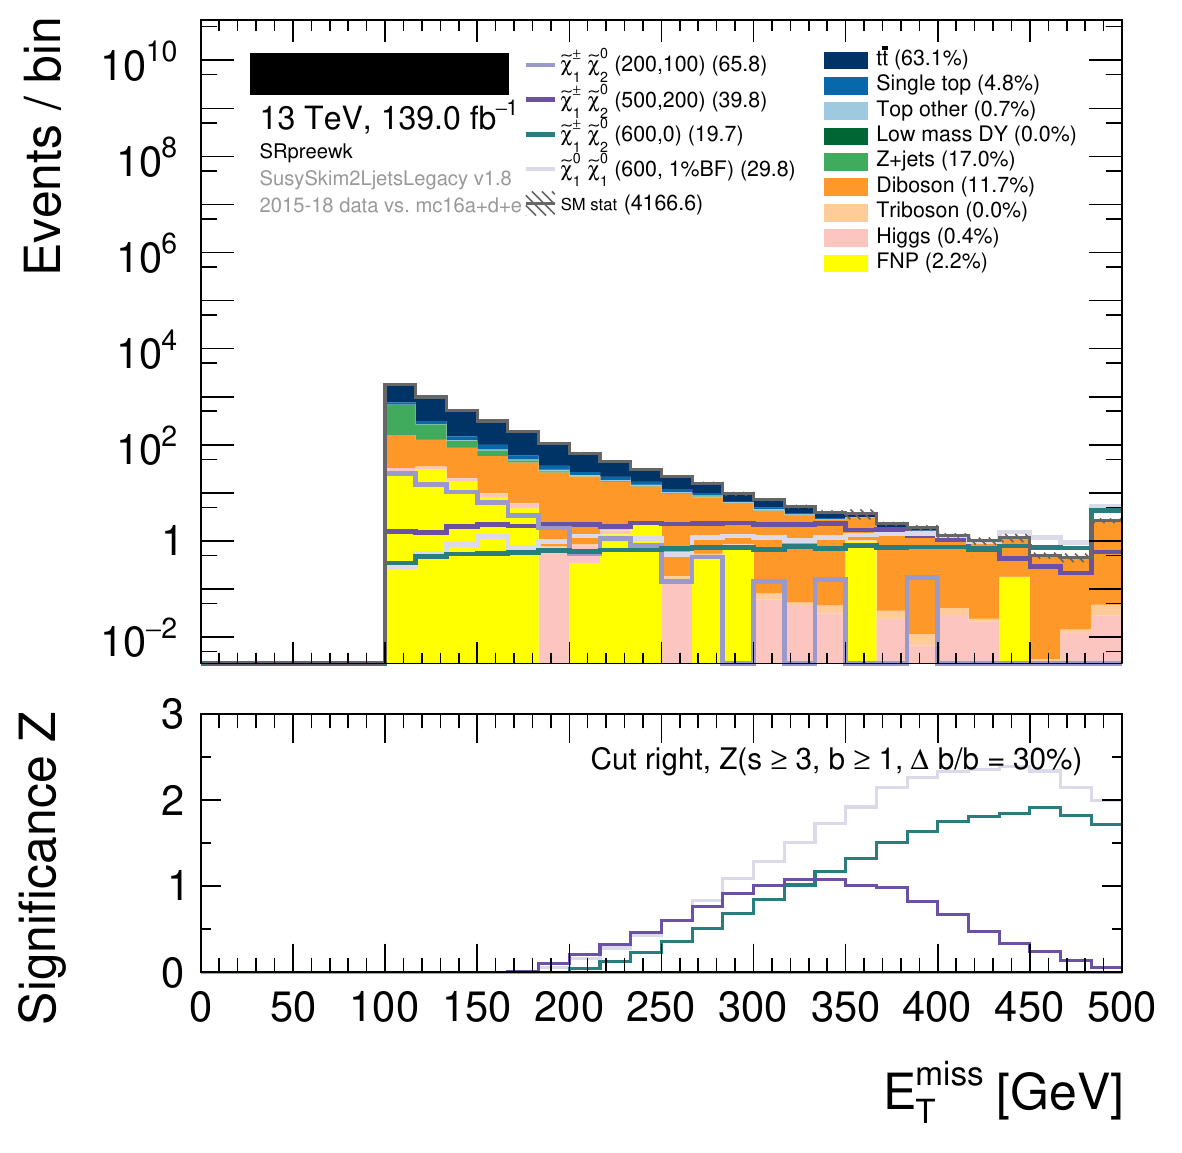
\includegraphics[width=0.49\textwidth]{figures/2ljets_presel_met_logy.png}
\hfill
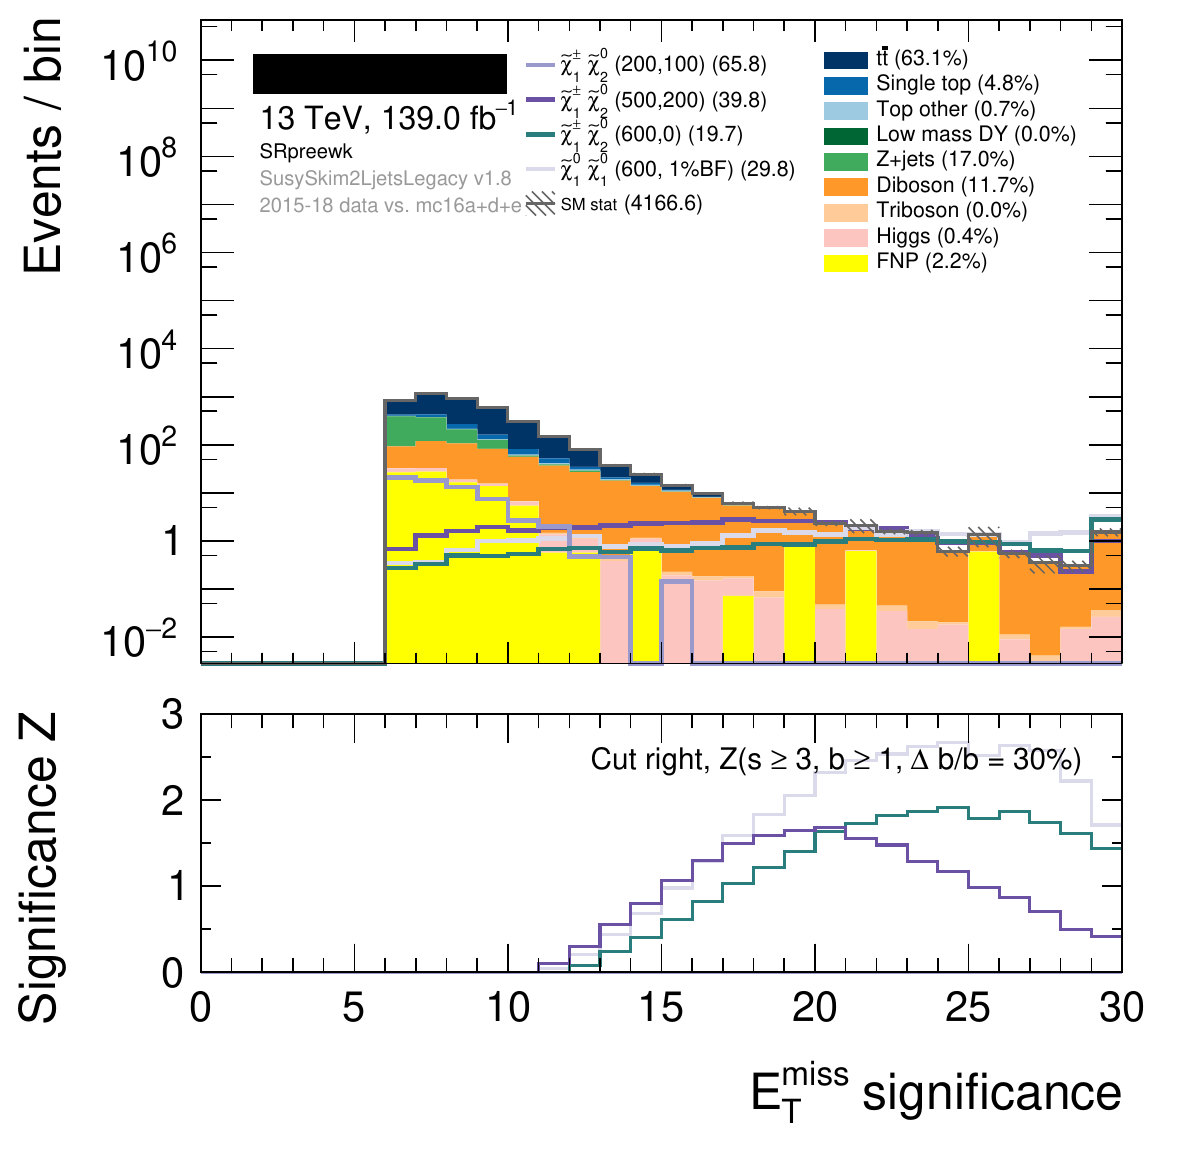
\includegraphics[width=0.49\textwidth]{figures/2ljets_presel_met_sig_logy.png}
\caption{
Illustration of how $\metsig$ beats $\met$ alone in sensitivity to
example signal models.
At large $\metsig$, $t\bar t$ and other backgrounds are suppressed, leaving
quite pure diboson backgrounds and greater significance measures.
Signal models with smaller mass splittings tend to have the bulk of their
events at smaller $\met$.
\\[0.5em]
This loose selection ``SRpreewk'' requires two same-flavor opposite-sign
signal leptons with
$\mll \in (71, 111)~\eV[G]$,
$\mjj \in (60, 110)~\eV[G]$,
$\nbtag \leq 1$,
$\met > 100~\eV[G]$, and
$\metsig > 6$.
\\[0.5em]
``Significance'' displayed in the lower subplot uses the Binomial significance
$Z_{Bi}$ from~\cite{cousins2008evaluation}, with a $30\%$ background
uncertainty and yields taken to the right of a given value.
Large values indicate expected sensitivity to the signal model.
}
\label{fig:2ljets_presel_met}
\end{figure}

Uncertainty in $\ptmiss$ is modelled for $\metsig$ by a covariance matrix, $S$,
in the transverse plane, and used to define
\begin{equation}
\metsig
=
\ptmiss S^{-1} \ptmiss
,
\end{equation}
which can be rearranged into a ratio of $(\met)^2$ to a function of elements
of the covariance matrix~\cite{atlas_met_significance}.
This is the square of a Mahalanobis (standard-deviations) distance between
the origin and $\ptmiss$~\cite{mahalanobis1936generalised}.

Just as $\ptmiss$ is constructed from a (negative) sum of contributions from
objects in an event,
$S$ is a sum of covariances assigned to those objects;
both means and variances add linearly.


\subsection{Stranverse mass $\mttwo$}
\label{sec:mt2}

Just as the slepton is a supersymmetric partner to a lepton, the stransverse
mass  $\mttwo$ is a partner to the `transverse mass' $m_T$
(to be defined shortly),
that is useful in searches for supersymmetric particles.

The stransverse mass of an event is a greatest lower bound on the mass of a
pair-produced resonance, that applies when each partner decays semi-invisibly.
For example, an on-shell $\tilde\ell^+\tilde\ell^-$ pair decaying as
$\tilde\ell^+ \rightarrow \ell^+ \neutralino_1
,~
\tilde\ell^- \rightarrow \ell^- \neutralino_1$ has
$\mttwo(\ell^+, \ell^-, m(\neutralino_1)) \leq m(\tilde\ell)$, plus some error
margin for experimental resolution.
Such cases are common since, R-parity conservation implies pair production,
and the idea that dark matter could comprise the lightest supersymmetric
particle motivates invisible decays.

Lacking direct observation of sleptons, $\mttwo$ remains useful in separating
standard model processes; dileptonic $t\bar t$ and $W^\pm W^\mp$ decays both
satisfy $\mttwo(\ell^+, \ell^-, 0) \leq m(W)$ (since $0 \approx m(\nu)$).
The $\twoljets$ electroweak search depends on this effect;
most selections require $\mttwo(\ell^+, \ell^-, 0) > 80~\eV[G]$, or similar,
to reduce $t\bar t$, $W^\pm W^\mp$ and $\tau^\pm\tau^\mp$ backgrounds.

To be precise, the stransverse mass explores how to split the observed
$\ptmiss$ between the two visible decay products in an event, and can be
defined as
\begin{equation}
\mttwo(a_\mu, b_\mu, m)
=
\min_{\vec p\,+\,\vec q\,=\,\ptmiss}
\max
\begin{Bmatrix}
m_T(a_\mu + \{\!\sqrt{m^2 - \vec p_T^{\:2}},\,\vec p\,\}_\mu)\\
m_T(b_\mu + \{\!\sqrt{m^2 - \vec q_T^{\:2}},\,\vec q\,\}_\mu)\\
\end{Bmatrix}
,
\end{equation}
in which $m_T^2(p_\mu) = p_0^2 - p_1^2 - p_2^2$~\cite{lester1999measuring}.
As an extension, one can assign different masses $m_p$ and $m_q$ to the
the two invisible products~\cite{lester2015bisection}.

Numerical evaluation of $\mttwo$ can be performed efficiently with interval
bisection algorithms, which seek the least resonance mass for which the
transverse masses allow any compatible missing momentum
assignment~\cite{cheng2008minimal, lester2015bisection}.
Public code for calculating $\mttwo$ is available as a Python
library~\cite{gillam2021mt2}, to which I contributed a faster and more robust
implementation of the bisection algorithm by
Lester and Nachman~\cite{lester2015bisection} during this project.

\subsection{Cheat-sheet}
Uncomfortably many event variables are used to define the regions of this
analysis.
To aid future revision of their meanings, definitions and references for these
variables are collected here.
\begin{itemize}
\item $\met$: missing transverse momentum
\item $\metsig$: object-based missing transverse momentum significance;\\
described in Section~\ref{sec:metsig}
\item $\ptjone$: transverse momentum of the hardest jet%
\vspace{0.5em}
\item $\mll$: invariant mass of the hardest two leptons
\item $\mjj$: invariant mass of the two hardest jets
\item $\mbb$: invariant mass of the two hardest b-tagged jets
\item $\mjetone$: mass of the hardest jet
\item $\mttwoll$: `stransverse` mass of the lepton pair with massless invisibles;\\
described in Section~\ref{sec:mt2}
\vspace{0.5em}
\item $\rll$: distance in $\eta\textrm{--}\phi$ between the lepton pair
\item $\rjj$: distance in $\eta\textrm{--}\phi$ between the two hardest jets%
\vspace{0.5em}
\item $\njet$: number of signal jets
\item $\nbtag$: number of b-tagged jets;
described in Section~\ref{sec:btagging}
\vspace{0.5em}
\item $\dphillmet$: azimuthal angle between the lepton pair and $\ptmiss$
\item $\dphijmet$: azimuthal angle between the hardest jet and $\ptmiss$
\end{itemize}
All of these are physical properties of particles or collections of particles.
Please remember that none is an exact or true value;
all are are estimates based on approximate reconstructions.
While this distinction is easy to drop in lax language, is necessary to
understand the shapes of noisy variables such as $\mjj$ and indeed the
existence of $\metsig$.


\FloatBarrier
\section{Design}

The most impactful decision in a search is the design of its regions.
Like all decision in life, these designs must be made to balance conflicting
and vaguely-specified desires, and are informed with incomplete information.

This section describes the designs and rationales behind the control, validation
and signal regions of the $\twoljets$ analysis.


Splitting regions on $\metsig$ is the core idea behind the design.
The basic motivation for this design are displayed in
Figure~\ref{fig:2ljets_presel_met};
$\metsig$ does better than $\met$ in separating background and signal
contributions.
But there is more --- $\metsig$ also decently separates signal models from one
another;
signals with larger mass differences in their decays to invisibles tend to have
larger $\metsig$.
Binning regions in $\metsig$ therefore also improves sensitivity to
individual parameter points and allows targeted selections on other, locally-relevant,
event variables.


% CRs go in with relevant SR category
\subsection{High}

\subsection{Intermediate}

\subsection{Low}

\subsection{Off-shell}

\subsection{Discovery}

\section{Modelling}
% TODO backgorund samples
% TODO matrix method fakes
% TODO GMSB reweighting
% TODO off-shell plus/minus split
% TODO generator filtering

\subsection{Fake/non-prompt leptons}

\section{Validation}

\section{Systematics}

\section{Results}


